%\documentclass{article}
%\documentclass[journal]{IEEEtran}
\documentclass[12pt]{report}
%\documentclass{acta}

\usepackage{graphicx}
\usepackage{amsmath}
\usepackage{gensymb}
\usepackage{xcolor}
\usepackage{tabularx}
\usepackage{colortbl}
\usepackage{caption}

\graphicspath{{./media/}}
\begin{document}

\setcounter{page}{0}
\thispagestyle{empty}
\captionsetup{justification=centering}
\begin{figure}
\minipage{0.32\textwidth}
    \center
    
\includegraphics[width=40mm]{pg_logo}
    \caption*{\footnotesize Gdansk University of Technology}
\endminipage\hfill
\minipage{0.32\textwidth}
    \center
    
\includegraphics[width=45mm]{mathmods}
    \caption*{}
\endminipage\hfill
\minipage{0.32\textwidth}%
    \center
    
\includegraphics[width=30mm]{laq}
    \caption*{\footnotesize Universit\`a degli studi dell'Aquila}
\endminipage
\end{figure}

\begin{center}
    \textcolor{white}{to separate}\\
    \Large{\textbf{Erasmus Mundus Consortium “MathMods”}}\\
    \vspace{10mm}
    \normalsize
    Double Master's Degree Programme in\\
    Mathematical Modelling in Engineering: Theory, Numerics, Applications\\
    \vspace{5mm}
    
    \small{In the framework of the}\\
    \small{Consortium Agreement and Award of a Joint/Multiple Degree 2013-2019}
    \vspace{5mm}
    
    \Large\textbf{Master's thesis}\\
    \Large\textbf{A genetic algorithm based computer program for generating initial structure of realistic polycrystalline materials for molecular dynamics simulations }\\
    \vspace{5mm}
    
    \large
    \begin{tabular}{ccc}
        $Supervisor$ & & $Candidate$\\
        Dr.Eng. Szymon Winczewski  & &  Rustam Akhunov 
    \end{tabular}\\
    
    \vspace{10mm}
    \small
    2016/2018
\end{center}


\author{Rustam Akhunov}


\tableofcontents

\begin{abstract}
The work dedicated to realistic polycrystalline structure generation. The structure is simulated as a Voronoi tessellation structure. Voro++ library is used for tessellation generation. The grain size distribution and grain orientatoin distribution are reached by using Genetic Algorithm (GA). The study is done in 4 steps: grain size distribution fitting, grain orientation distribution fitting, grain filling by particles, relaxation. For grain size and grain orientation distributions and also for first step relaxation GA was used. Relaxation consists of two steps: first by using GA and second by removing excess atoms. By the end of structure generation relaxation within LAMMPS simulation software is done. In LAMMPS molecular static and molecular dynamics relaxation is done. All works are done on Gdansk University of Technology's supercomputer.
\end{abstract}


\section{Introduction}

There are known a lot of modern applications of polycristalline materials. Polycristallines are used for tritium generation \cite{john99}, automotive, healthcare and non-destructive testing \cite{pardo11}, solar cells \cite{schrop98}, semiconducting elements \cite{harb85} etc. With increasing demand of new properties of new materials increases also need for the modern methods of polycristalline simulation \cite{shen15}. And this work is one more attempt to deal with the simulation of polycryrstallines in molecular dynamics environment such as LAMMPS \cite{plimp95, plimp00}

There are numbers of experiments and theoretical researches for the intrinsic structure, effective thermal conductivity, lattice dynamical, optical and thermodynamic properties of polycristalline \cite{shen15}. But still many characteristics have not been researched sufficiently.

We know few methods for generating digital nanostructured materials for use in the simulation: Poisson–Voronoi tessellation (PVT) \cite{wear86}, Monodispersive grain size (MGS) \cite{wang96}, Laguerre–Voronoi tessellation (LVT) \cite{fan04}, Johnson–Mehl (JM) model \cite{okabe00} etc. In this work Voronoi tesselation model is used for the reason of its good solution for the complex sctructural nanocrystals and also convinient interface for the genetic algorithm, that is used during polycristalline generation. It is also generally accepted that many single-phase fully dense nanocrystals are described by a log-normal grain size distribution. And this distribution is considered as a reference for polycristalline generation.

The goal of this work is implementation of general methodology and usable tool of generation realistic polycrystalline structure. It should correspond grain sizes and orienation distribution, have minimal energy and be relevant to experimental density, lattice constant etc. The methodology also should be fast enough in order to do generation in one or several days on adequate resources. This everything was done based on existing results for different polycrystallines.

\section{Overview of existing methods and results}

Before starting the research an overview on existing results in several related papers is done. One of the most important article for this research was "Constructing three-dimensional (3D) nanocrystalline models of $ Li_4SiO_4 $ for numerical modeling and simulation" \cite{shen15}.

In this paper authors consider problem of generation $ Li_4SiO_4 $ polycrystalline. In fact narrowing the result only for $ Li_4SiO_4 $ polycrystalline is the main limitation of this study. But in current work it was tried to implement more general approach. Of course by making more general method one can face much more problems with efficiency and time consuming of the generation method. But this general method can be adapted to the particular element. And having such a method can simplify the whole task for particular element and help researcher concentrate only on specific features of chosen matter.

The authors use genetic algorithm to reach particular distribution of grain sizes and as one can see they use only mutation operator without crossover. But in this work in contrary both mutation and crossover operators are used. Moreover, 3 variants of crossover and 3 variants of mutation were implemented in current study in order to find optimal operators for the task. It were performed numerous computing experiments and optimal combination of operators and other algorithm parameters were chosen.

But it is necessary to pay tribute to the good results obtained during implementation of the algorithm in the above article. Authors were able to reach very good permormance. In particular, the computation time per step was 3.7 s with 6 processors and it is much better compared to the result 3.9 s with 32 processors \cite{suzudo02}.

Another interesting paper dedicated to the problem is "Lattice models of polycrystalline microstructures: A quantitative approach" \cite{rinaldi08}.

Here authors refer to available methods for creating polycrystalline structure. Among several different approaches they mention Voronoi tessellation as a good method for obtaining a polycrystalline structure. It is noticed that this method is very popular and wide spread in fitting to the experimental data and therefore presented in special commercial software such as AMIRA, MIMICS, SURFDRIVER.

Of course Voronoi tesselation method has disadvantages like that it represents only convex polyhedra that is not true for real polycrystals. It is also known that real grains are not necessary polyhedra at all. Nonetheless, Voronoi tessellation remains very quick and reliable method of generation structures close to the real polycrystalls. 

In the paper it is also noticed that instead of focusing on precise microstructure it is much better focus on major statistics like  distribution of grain size and grain orientation. It is actually what is done in current study.

However, in the paper the main goal is achieving the mechanically equivalent polycrystalline. Although this approach is good for mechanical properties of material it loses any other aspects of real matter. That reason leads that these results cannot be fully adapted for current research.

Another significant result in realistic generation of polycrystalline structure was achieved in "Mechanical properties of polycrystalline graphene based on a realistic atomistic model" \cite{kotak12}.

Here authors did great work in order to obtain realistic atomic structure of graphene. They implemented algorithm for atomic structure generation based on the growth principle. It means that after random location of grain centers they tried to simulate growth of grains by considering borders of growing grain step by step. They also followed misorientation distribution that have one to one correspondence with orientation distrubution. It is also emphasized the importance of realistic simulation of grain boundaries because of their significant impact on mechanical and electrical properties of material.

The main disadvantages in the work is that the result is valid only for graphene and graphene like structures. There is also problem with algorithm used in the paper. This approach needs more computing resources and have some difficulties in parallelism. Usually such structure construction needs days for obtaining usable results if the system has usual for simulation sizes (millions of particles). The real distribution of grain sizes is absolutely neglected in the paper. It is considered only uniform distribution for the grains that does not follow most of real structures. But nonetheless, some ideas for misorientation distribution were taken for work described in current thesis.

In following "Studying the elastic properties of nanocrystalline copper using a model of randomly packed uniform grains" \cite{guo13} paper an interesting new approach in studying mechanincal properties of nanoscaled polycrystalline materials was found. Authors offer to concentrate on finding dependency of elastic module on grain boundaries and therefore they make artificial ideal polycrystall where they obtain uniform grain sizes that is not true for most of realistic structures.

The last very interesting paper to talk about which was considered during literature overview was "Generation of 3D polycrystalline microstructures with a conditioned Laguerre-Voronoi tessellation technique" \cite{falco15}.

Here authors got really singnificant results in obtaining very close to real size distribution polycrystalline structure. In order to do this they used extended Voronoi tessellation method so called Laguerre-Voronoi tessellation already mentioned above \cite{fan04}. They implemented procedures that allow to associate particles' weights with the grains sizes. This method helps to obtain very realistic distribution of grain sizes and use it in the following simulation that they actually did. During simulation using this kind of tessallation they compared simulation results with real experiments with annealed aluminum. Obtained results show high efficiency of this approach and can be used in our work too. Thank to developer of Voro++ library this tessellation is already implemented in the library and one can use Laguerre-Voronoi tesselation as first approximation in genetic algorithm. It can significantly improve time of calculation.

Above articles were just theoretical statements with some obtained results. But it is also important to consider some practical software that currently exist and can help to generate polycrystalline structure.

Firstly, I would like to mention very useful modern software so called nanoSculpt \cite{prak16}. It allows to construct atomic structure inside any shape and form. It also supports constructing of Voronoi tessellation for polycrystalls in any shape. It was written using C language and quite easy extensible. But unfortunatelly, currently this package does not support user defined particular distribution of grain size and grain orientation during costruction of structure. 

Another interesting tool is AtomEye \cite{juli03} developed by MIT staffs. It is very comprehensive and powerfull tool for dealing with atomic structure. One of the most interesting utility in this package is so called voronoirize tool. It can be used for building polycrystalline structures. The software is written in C language and this might be considered as advantage. But it has same problem - it does not follow user defined distributions of sizes and orientations. 

And the last tool that is mentioned in current work is Atomsk \cite{hirel15}. According to the website title of the utility it is the Swiss-army knife of atomic simulations. It supports many and many methods for atomic simulation. One can obtain numereous output format for any simulation programs one need. But one will face the same problem as in mentioned above tools. To generate polycrystalline structure with particular distribution one needs to define orientation and size for each grain by hand. It is not convinient in particular with big sized simulation boxes. Moreover this utility is written in Fortran language that is not very convinient tool for wide support and extension. Particularly in industry field.

As one can notice there are many researches and tools dedicated to the problem of generating of polycrystalline structures. But there are several problems that one can face while using them. Firstly they do not support generation based on user defined distribution that makes these tools very hard to use in realistic conditions. Secondly, tools and methods which support realistic structures work on very slow algorithm that needs days for obtaining trustful results. Thirdly, sometimes tools are written in "not good" languages and are hard to maintain.

These all reasons inspired this study to create useful tool for generating realistic polycrystalline structure written in C++ language and backed by LAMMPS simulation software. For Voronoi tessellation method Voro++ library is used.

\section{Building the Voronoi tessellation}

As it was mentioned above Voronoi tessellation for building polycrystalline structure is used for this work. But for obtaining real stucture one has to fit some properties of natural crystalls during generation of tessellation. In this work special interest dedicated in fitting tessellation to the two crucial distributions: grain size distribution and grain orientation distribution. All generation done in periodic condition of the boundary.

\subsection{Grain size distribution}

Grain size distribution depends on many characteristics of polycrystal growth (velocity of crystallization, extra magnetic field etc) and environmental factors (temperature, pressure etc). It is widly beleived that in general any grain size distribution in polycrystals for most cases can be fitted to the lognormal function \cite{shen15, liu14}:

\begin{equation} \label{lognormal}
f(x) = \frac{1}{x} \frac{1}{\sigma \sqrt{2\pi}}exp(-\frac{(ln(x) - \mu)^2}{2\sigma^2})
\end{equation}
\bigbreak

As one can see there are only 2 parameters that can influence distribution shape $ \sigma $ and $ \mu $. Environmental characteristics can change these 2 parameters and impact on grain size distribution. Of course, there are plenty other types of grain size distribution like bimodal lognormal distribution, uniform distribution and so forth. But in general, type of distribution does not affect to the research made in the current work and this is why just simple lognormal distribution is considered as a reference. Moreover \ref{lognormal} is used as a fitting function for the grain size distribution in overwhelming majority of scientific papers regarding polycrystalline structures \cite{shen15, liu14}.

The reason why one can be interested in the grain size distribution is that this polycrystalline matter's feature has direct effect to the mechanical and electromagnetic properties of the polycrystalline structure. And very often just knowledge of an average grain size cannot give us specific parameters of the material. In research about effect of grain size distribution on mechanical properties \cite{terada10} one can find dependency of yielding on the grain size distribution. In the paper annealed aluminum is considered. Depending on annealing temperature and lubrication authors obtained different grain size distributions and therefore different stress-strain dependency hence different yielding, though average grain size is the same for all specimen.

Grain size distribution can be expressed as a dependency of appearing frequency on the grain size. But grain size can be interpreted in few different ways. In paper one can find grain size as volume of grain, area of the surface of the grain, simple area in case of films (2D nano-objects) or grain diameter (sometimes radius). In this work diameter of a grain is chosen as a meause for the distribution. Moreover to make all evolutions dimensionless normalized grain size is used. Normalizing is made by dividing grain diameter with average grain diameter across all grains of the material. 

An aim for the given work is to build some structure close to the given distribution (unimodal lognormal in this case). And one need to become familiar with popular methods of achieving some particular distributions.

Monodispersive grain size model \ref{wang96} implies attempt to simulate polycrystall by identically-shaped rhombohedral grains. The main purpose of such simulation just research of some boundary effects. Of course such a model does not reflex the real structure.

Poisson–Voronoi tessellation \ref{wear86} and Laguerre–Voronoi tessellation \ref{fan04} models are improvement for the classical Voronoi tessellation. These methods allow to fit some given distribution directly to the tessellation generation process. The methods are extremely fast compared to genetic algorithm described below. There is a problem though, one obtains distribution similar to the reference distribution, but the distribution not close enough to be able to say about dependency of particular distribution and material properties. However these approaches can be used as an extremely good first approximation for genetic algorithm.

Classical Voronoi tessellation backed by genetic algorithm is comprehensive and relatively modern method for polycrystalline structure generation. It is used here in work and will be discussed in detail below.

Because of simplicity of implementation, low resource demanding, relatively fast computation and a few other advantages of the genetic algorithm method it was chosen as the only method for the generation not only grain size distribution but also orientation distribution and first level of relaxation of the structure. 

\subsection{Genetic algorithm for the grain size distribution}

There are several key elements and terms needed to define before implementation of \textit{\textbf{genetic algorithm}} (GA). First of all when one refer to the GA it is needed to understand what is \textit{\textbf{individual}} for the current task. In case of current work one deals with the Voronoi tessellation. Voronoi tessellation, in its turn, deals with a set of 3D points in the space so called seeds or generators. Thus the object that holds these seeds will be considered as an individual for the task. Remember that individual represents a solution for the given problem and in case of current research the right individual will generate correct polycrystalline structure hence solve the given task.

The set of individuals is called \textit{\textbf{population}}. The \textit{\textbf{size of population}} is the number of individuals in the set. Population in some fixed time is called generation. The first generation influences strictly on the speed of GA's convergence. And not only speed but also problem of stucking in local minima also depends on initial population. Therefore strategy regarding forming initial generation can significantly impove GA. In this work uniform, i.e. random generation of individuals is chosen. It helps to cover space of solutions independently and bypass local traps. Of course, the size of population is also important for good peformance. But this parameter will be chosen later based on calculation experiments.

Another crucial term of GA is \textit{\textbf{genome}}. Genome consists of genes and genes reflect some properties of the individual. In this work each 3D seed is considered as gene and the whole set of seeds for given individual is a genome. So, all further manipulations in GA will be done on set of seeds.

In order to be able to manipulate genes one needs to encode them, convert from genotype to so called \textit{\textbf{phenotype}}. It was chosen real number encoding for the seeds coordinates because it is natural and convinient representation of the 3D points. Each point is represented by set of 3 real numbers: x, y, z coordinate of corresponding 3D point. The whole genotype is kind of 2 dimensional array. First level of array has size of number of individuals. The inner level has size 3 - the number of coordinates. Thereby there is 3*N sized array representing an individual.

The \textit{\textbf{fitness}} is characteristic of individual showing the approximation of indvidual's phenotype to the objective function. It is another important term that has to be defined. Instead of fitness calculation it might be calculated inverse value so called \textit{\textbf{fitness penalty}}. It shows the same, how far or close the individual's phenotype to the defined function by taking some difference between expected and current values. In this work fitness penalty calculated by formula \cite{shen15}:

\begin{equation} \label{penalty}
W^2 = \frac{1}{N} \sum_{i=1}^{N} [P_r(d_i) - P(d_i)]^2
\end{equation}
\bigbreak
 
where N - number of points where penalty is calculated, $P_r$ is size-distribution of individual, P is expected size-distribution (fitting function), $d_i$ is point where penalty is calculated.

The size-distribution of individual is constructed by dividing whole interval of possible grain sizes into equal-distant subintervals - bins. For each bin number of grains with size within this interval is calculated. This amount of grains is divided by total number of grains in individual to obtain normalized frequency. Hence, N is the number of bins on which the whole interval is divided.

The expected size-distribution in this study is lognormal distribution. Each point where value of distribution is calculated is the center of the bin.

The formula \ref{penalty} was chosen for the reason of fast convergence of GA with such a penalty function compared to several other meausers \cite{shen15}. Hence, convergence of GA in context of penalty function is tendency of penalty function's value to zero.

Before moving to the discussion about GA operators it is needed to mention about \textit{\textbf{breeding}} and new population \textit{\textbf{selection}} strategies that are used in this work.

\textit{\textbf{Breeding}} is the process of generation of new population candidates. It can be done by many different ways but in this work crossover and mutation operators are used for this purpose. After obtaining initial population the cycle runs to obtain all further generations. In this cycle successively crossover and mutation are applied. This procedure gives candidates for the new generation. New candidates are mixed in common pool with the current population. The new population is selected based on individuals' fitness penalty. Best individuals go to the next generation and the process repeats until \textit{\textbf{stop criteria}} is reached (will be described later).

The described breeding strategy was selected because of its simplicity and relatively ease of implementation. Furthermore it is classical scheme for the GA. Described selection strategy was chosen for the reason of guarantee of improvement of population from generation to generation.

As was mentioned, two classical operators are presented in this implementation of GA for size distribution. \textit{\textbf{Crossover}} operator is an operator allowing to mix up genomes of the individuals (parents) with the same analogy as crossing within species in nature. \textit{\textbf{Mutation}} operator is an operator allowing to generate new genomes (bring new information to the population) by changing somehow some part of genomes in individual.

Crossover operator can be of different implementations but all implementations include two main elements: individual selection and crossover procedure. It worths to mention, that selection of individual for crossover and selection individuals for a new generation are absolutely different operations.

There are number of selection for crossover strategies that will be discussed here. Classical selection for crossover \textit{\textbf{roulette wheel}} selection is not good choice for GA in current situation. Roulette wheel selection is very noisy and the rate of evolution strictly depends on the variance of population fitnesses. Another selection strategy is \textit{\textbf{random selection}}. It is even more disruptive than roulette wheel and therefore it is also not acceptable. \textit{\textbf{Tournament selection}} is the best variant for the current task. Competetion between individuals and random selection of individuals for the competitions bring selection pressure, which drives GA to get better fitness for the next generation. Finally, tournament selection was chosen for the GA implementation.

\textit{\textbf{Crossover}} procedure consists of two parts: cross site random selection and swapping genes between individuals following the cross site. Cross site selection might be one-, two- or multi-point. In this work it was used one- and two-points crossover because of it simplicity in implementation and good influence on the evolution rate. Uniform crossover is also implemented for diversity purpose and for ability to check how crossover operator impact on evolution rate and convergence of GA.

In case of Voronoi tessellation's seeds it is necessary to define how evalute cross site selection. The seeds are 3D points in the space and therefore one can determine cross site as a plane dividing individual's volume into two parts in case of one-point crossover. In case of two-point crossover one needs 2 cross section planes and so forth for multi-point crossover. One-point crossover is selected as an operator for the current study therefore it is needed to find only one cross section plane. But the problem that to find such a plane you need to take into account problem of dividing individual's volume to the parts with the same number of particles (seeds). When you divide 2 volumes with randomly located seeds there is not guarantee that your division will be successful and corresponding parts of 2 individuals will contain equal amount of seeds. Even when one will try to adjust the plane to make division useful (bring it to such a condition that respective parts of individuals have the same amount of particles) and change the angle and/or shift of the plane it is much more probable that one will fail in such refinement (see Figure \ref{faildivision}).

To avoid problem with planes seed-to-seed mapping approach was introduced. Seed-to-seed mapping is some association between seeds of one individual with seeds of another individual. The association for this study is made based on distance between seeds of two individuals. The distance was calculated after overlaying two sets of seeds in one volume. It's calculated only between seeds from different individuals. Example of such association is on Figure \ref{mappingindividuals}.

\begin{figure}
    \centering
    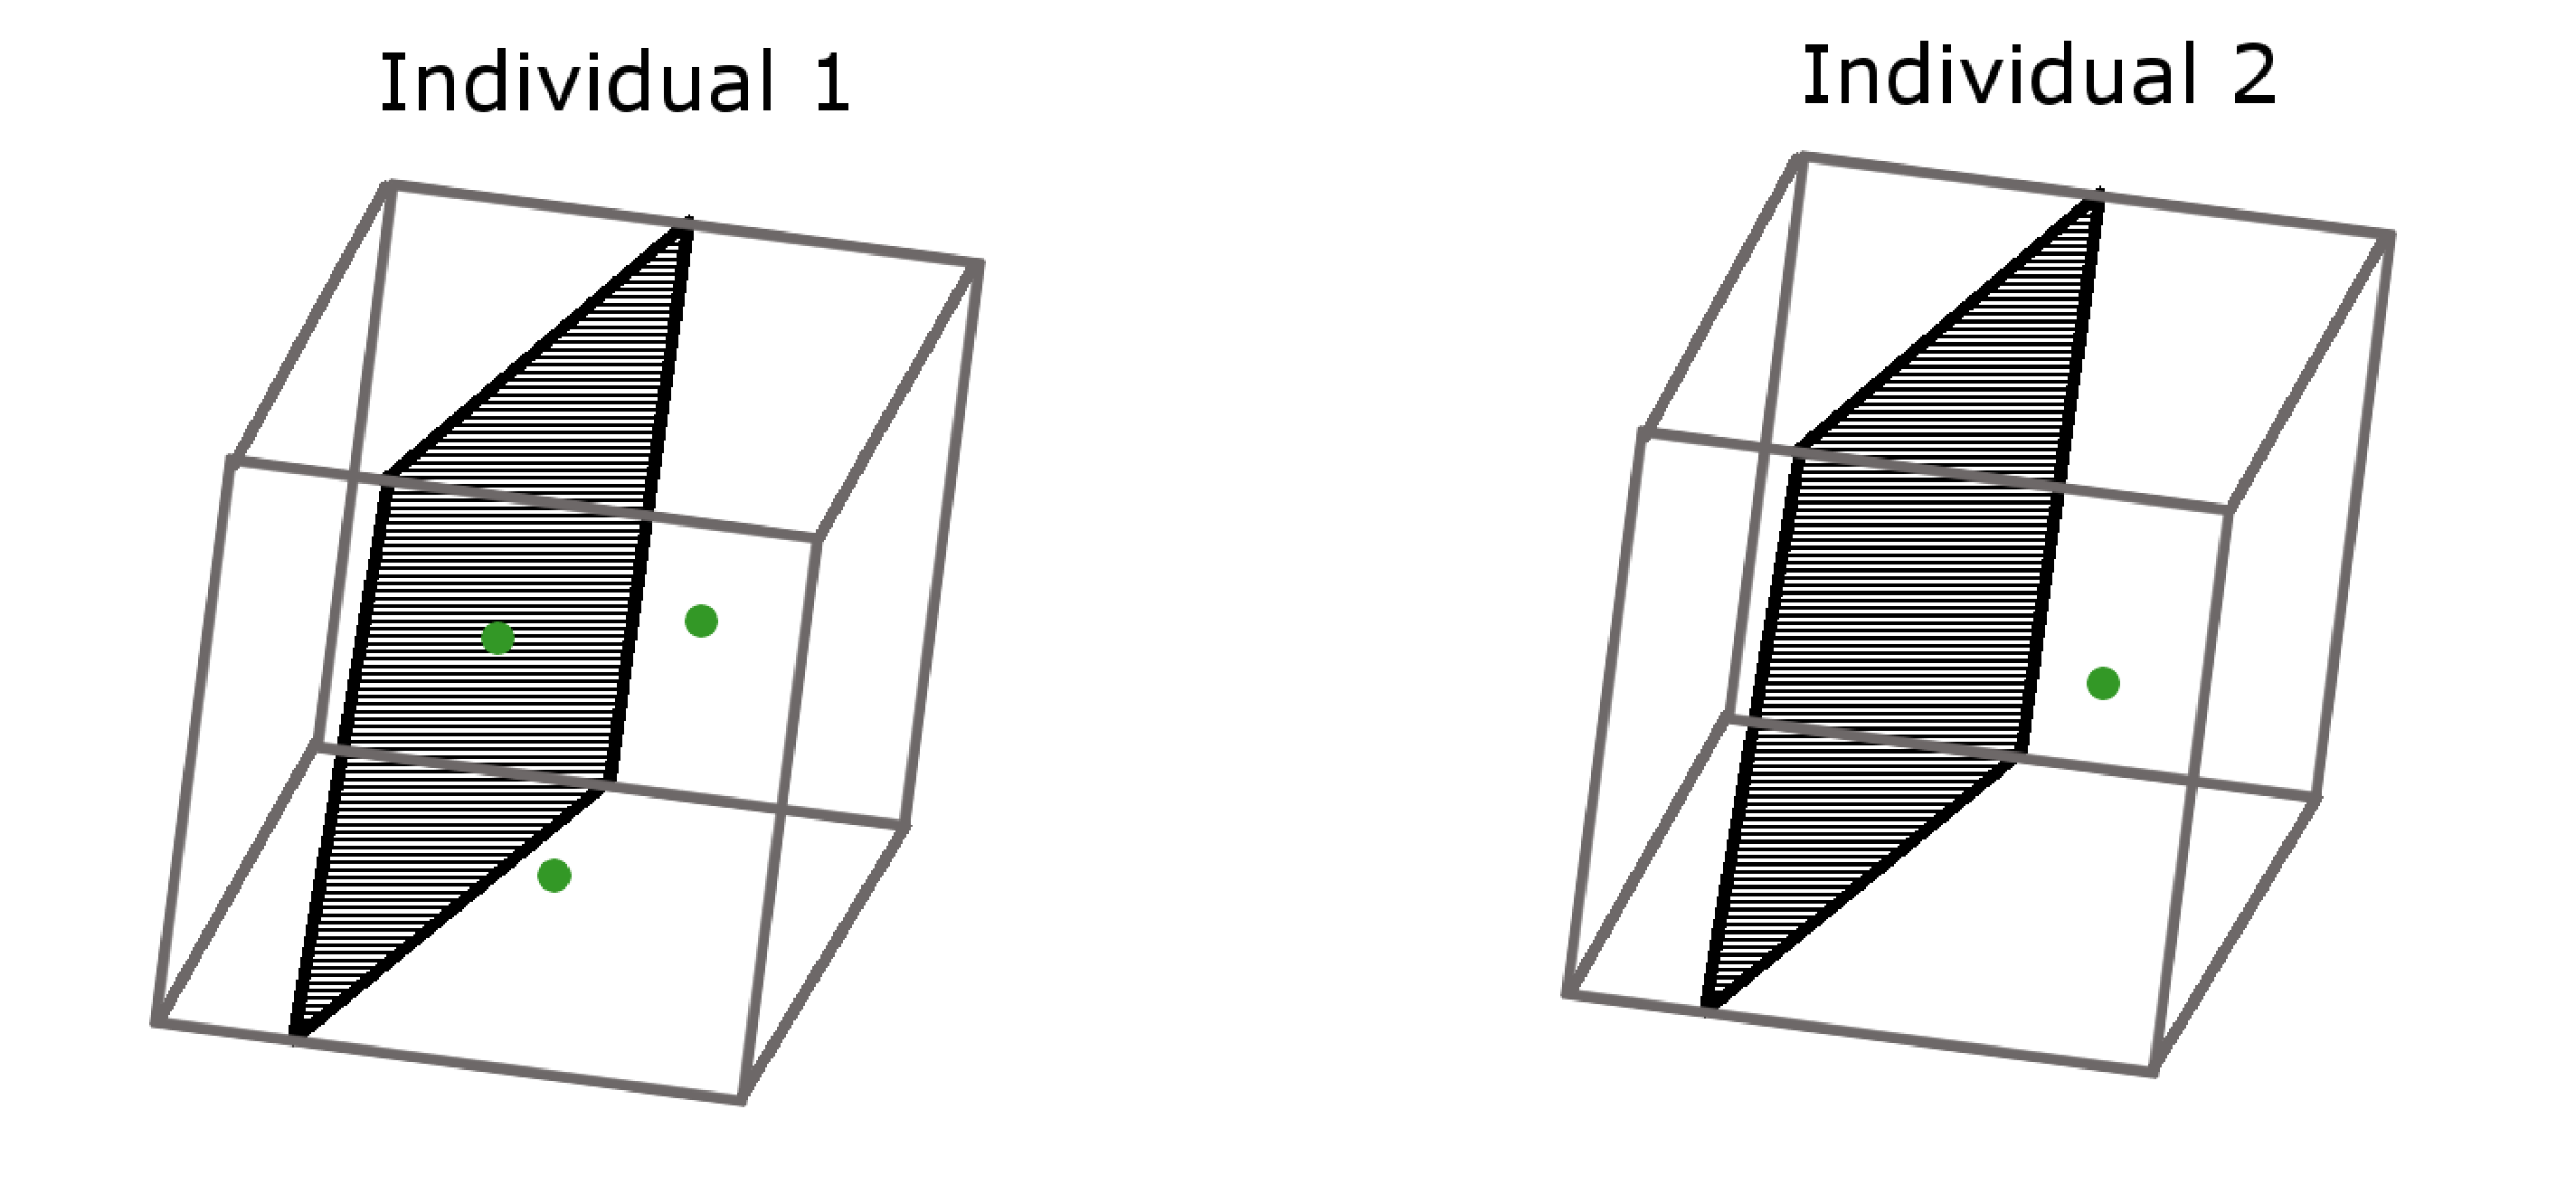
\includegraphics[width=3.0in]{cubes_cross_section}
    \caption{Cross section plane very rarely divide individuals' volume into parts with equal amount of seeds}
    \label{faildivision}
\end{figure}

\begin{figure}
    \centering
    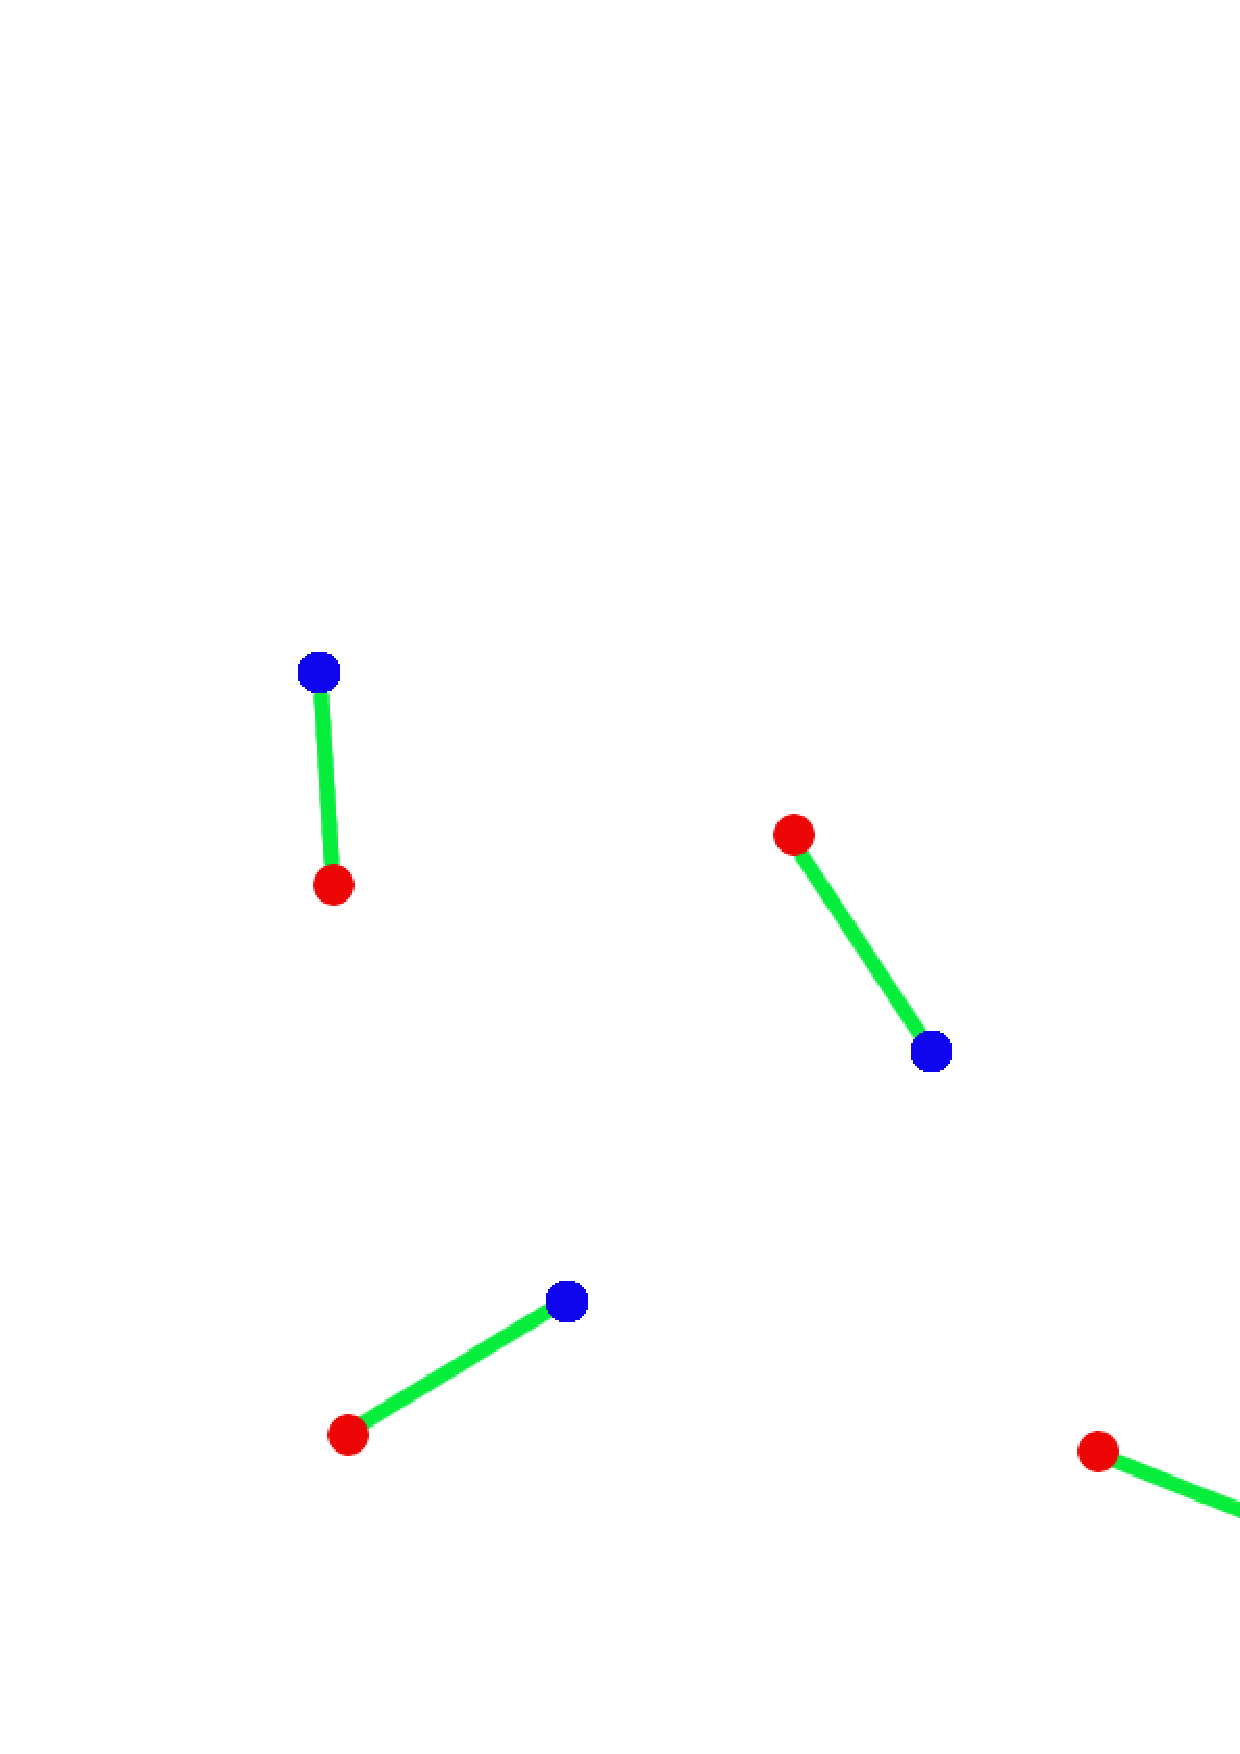
\includegraphics[width=3.0in]{individuals_map}
    \caption{Mapping of two individuals' points. Blue colored dots are points of first individual and red ones are of the second individual. Pairs are made of points from first and second individual according to the shortest distance between them. Green lines show which points are chosen for pairing. Each case of pairs is made between closest points.}
    \label{mappingindividuals}
\end{figure}

\begin{figure}
    \centering
    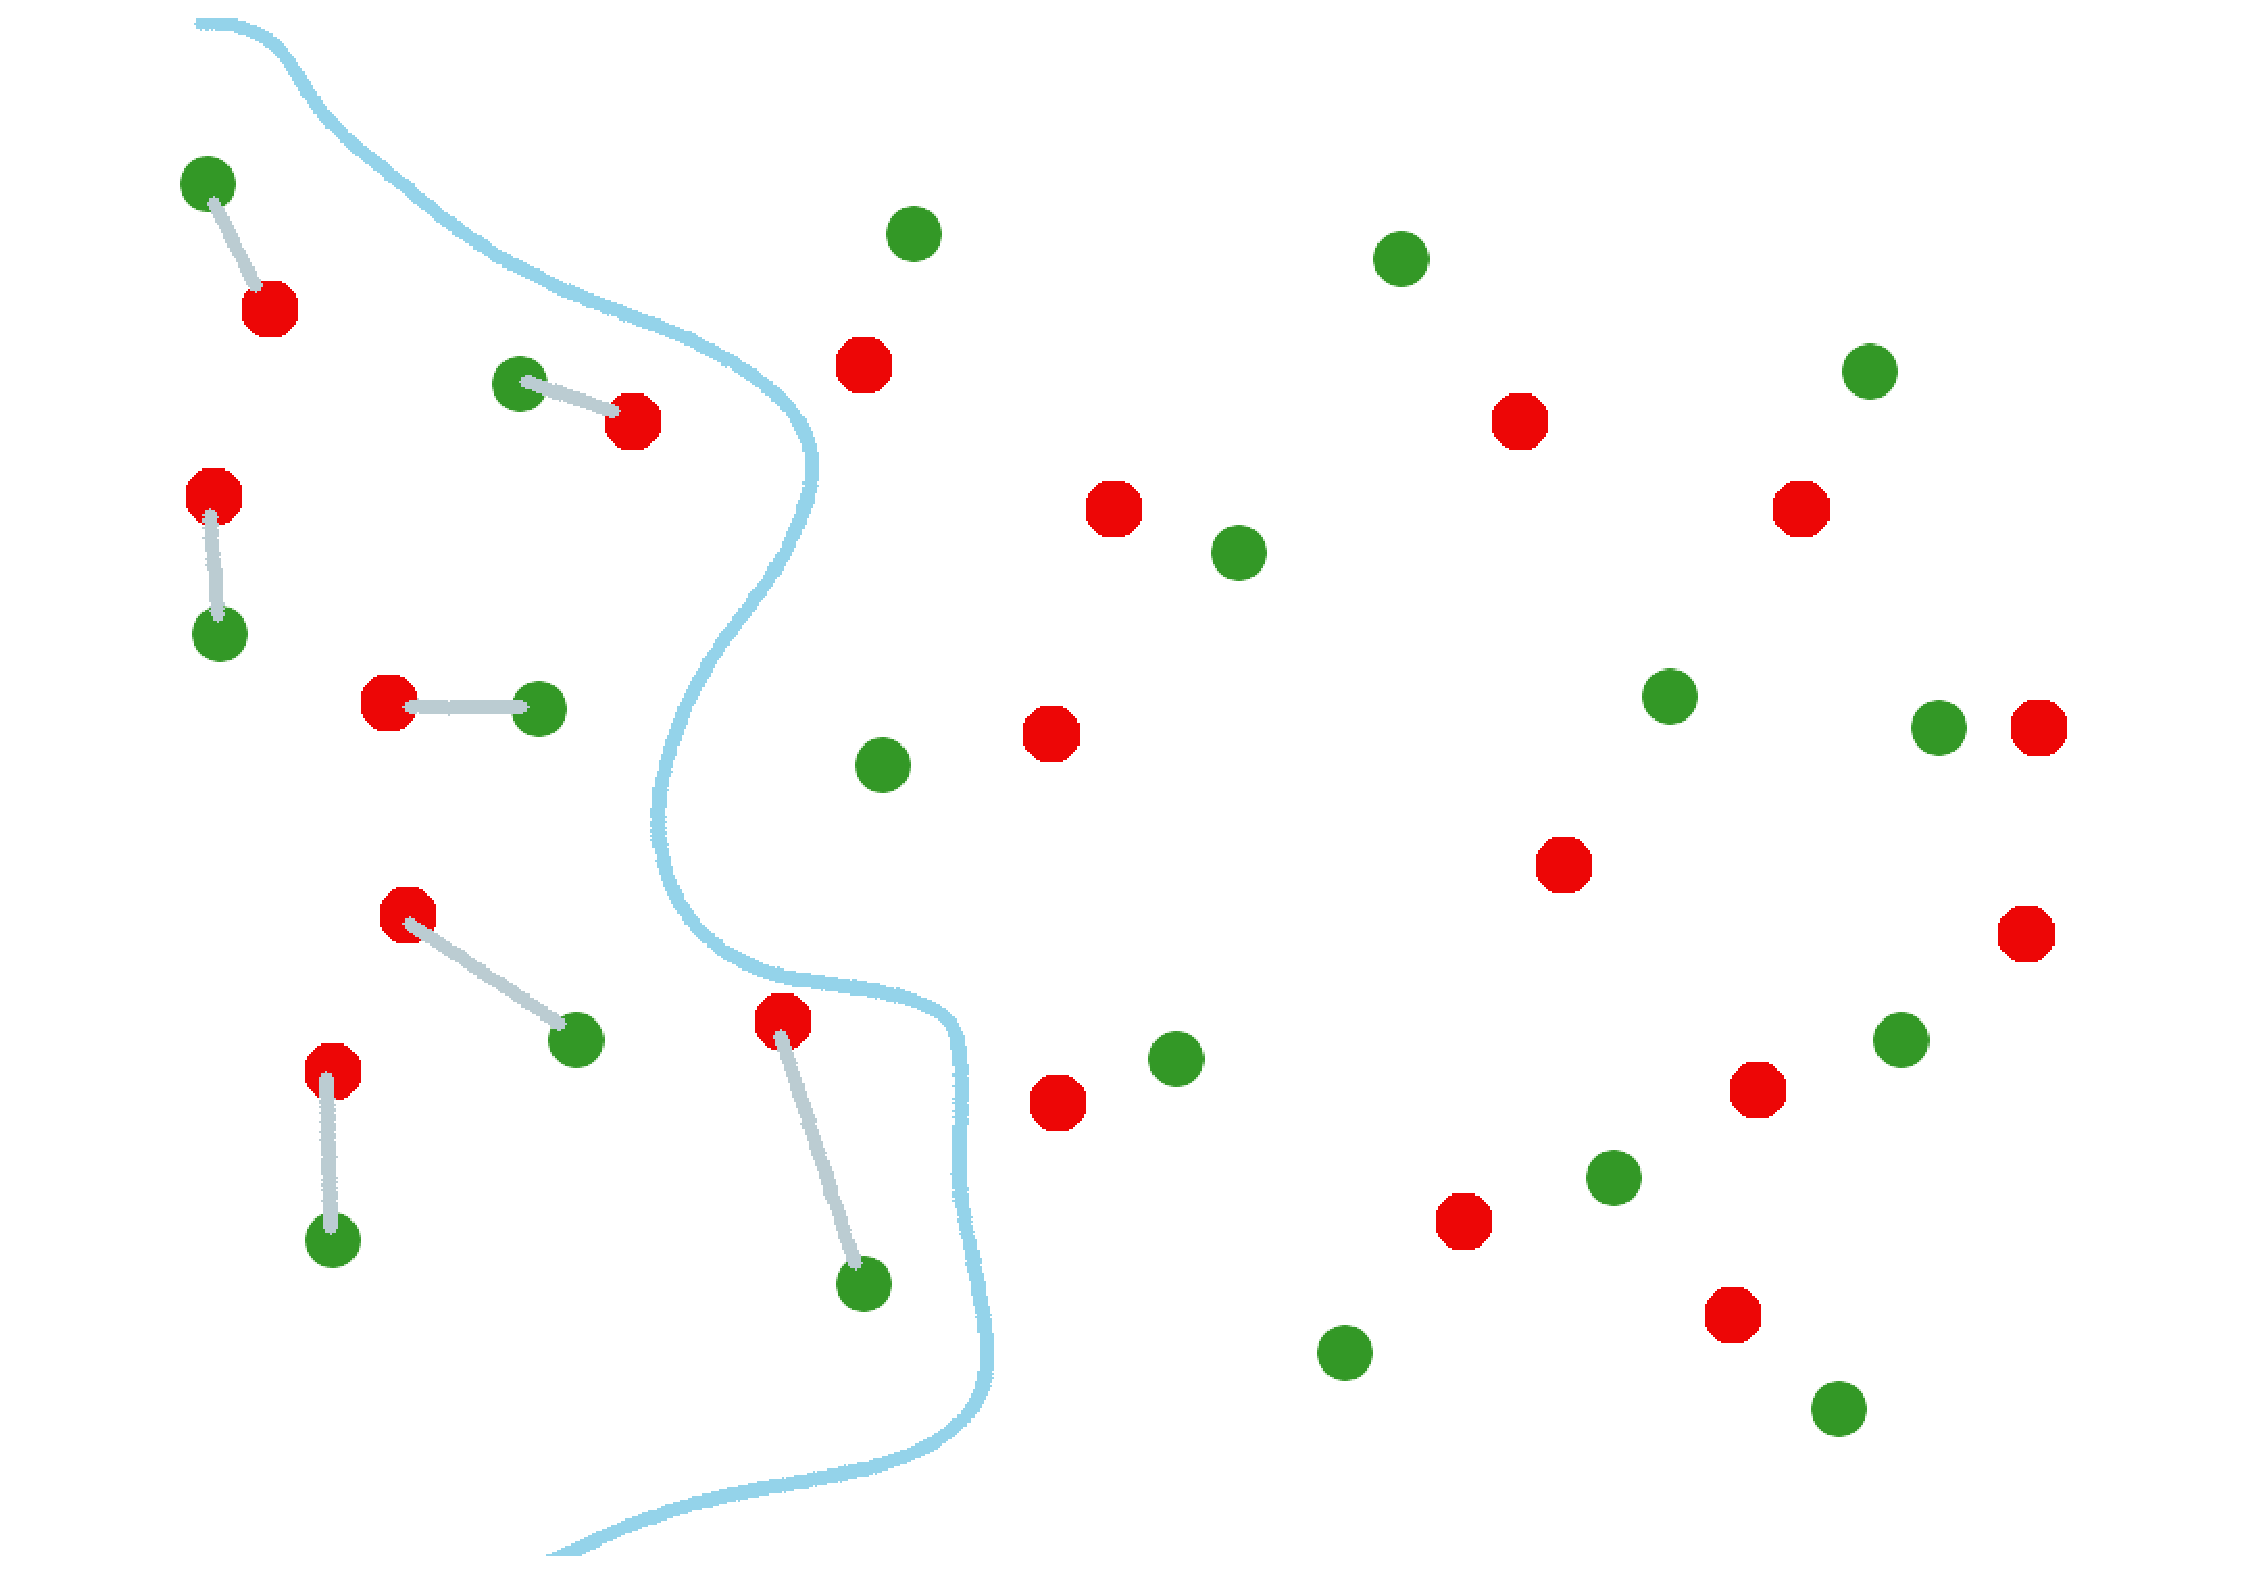
\includegraphics[width=5.0in]{3d_map}
    \caption{Freeform volume used for crossover. One type colored dots are seeds from one individual, another type colored - from another individual. Light gray lines are pairing of seeds. Blue line is freeform cross site.}
    \label{3d_map}
\end{figure}

After obtaining such a map between seeds it is easy to choose cross site for crossover. But now cross site is not a cross section plane but it is kind of free form surface that wrap some equal amount of seeds in both individuals. Equality keeps because of calculated mapping between seeds (see Figure \ref{3d_map}). One needs just choose randomly initial point for crossover. Then it is necessary to choose some defined number neighboring seeds in one individual and interchange seeds between individuals according to the mapping. Of course, such a mapping is not unique because one can have cases with equal distances between one seeds from one individual and several seeds from another individual. This problem is solved just by selecting random neighboring seed among similar minimal distance seeds and if seed is already used in map it skiped and new nearest seed is searching (with exclusion of already busy, paired seeds).

Having such a mapping between seeds it is possible to perform two-point crossover. It is needed just repeat procedure for one-point crossover two times on the same parents.

Uniform or random crossover is made by random choose of points for the offspring either from one individual or from another one.

So far, the discussion about crossover operator was in condition that one deals only with 2 individuals for each turn. But this operator can be not only for two individuals (parents) but also for three parents and even more parents. This type of operators as many other variants like Precedence Preservative Crossover, Partially Matched Crossover etc. are more complicated in implementation and very hardly predictable. This issue predetermined choice for current implementation.

\textit{\textbf{Mutation operator}} helps to bring new information to the generation. It works similarly to mutation in the nature. Individual has genes and mutation operator changes some of the genes and thereby help to bypass local minimas by extending search space. Number of genes that is changed due to mutation defined by \textit{\textbf{mutation probability}}.

Mutation operator can flip bits if genome encoded by binary string. But in case of 3D seeds it is not applicable. Exchange of genes when one part of genome interchanged with another part of the same genome is also not acceptable because it narrows diversity and can negatively affect on evolution rate. The same results come from reversing but it is valid only for bit encoded genome. The best choice for current study is just slight change of coordinates of seeds. Character of coordinate's changing produce parameters that will help to adjust operator behavior to the given task. These parameters will be discussed later. Another possibility to implement mutation is just reinitialization of seed. How many seeds will be reinitialized depends on mutation probability.

As was mentioned mutation operator was implemented as an operator that just shifts coordinates of seeds with some given probability. It is important to define maximum shift value that can be performed during mutation. One can take some fixed value for the shifting. This approach has a disadvantage because one needs to change the fixed shifting any time when sizes of simulation volume change. Another approach is to bind shifting to the dimensions of volume so it would be automaticaly adjusted to any volume. In this work adjustable approach is chosen. It is done by using average volume per seed. This value is pretty simple:

\begin{equation} \label{avgvolume}
V_{average} = \frac{V}{N}
\end{equation}
\bigbreak

where V is volume, N is number of seeds.

Average volume can be used for calculating shifting by taking cubic root from its value, i.e.:

\begin{equation} \label{shift}
d = \sqrt[3]{V_{average}}
\end{equation}
\bigbreak

This value is auto-adjusting to the given volume and you have guarantee that you will not go far out of volume when you perform mutation. It is important because big amplitude of shifting can cause of not convergence of GA.
 
If one has all necessary elements for GA it is important what is \textit{\textbf{stop criteria}} for GA. When it should stop its evoluations. There are several classical conditions for GA stop. 

- \textit{\textbf{Maximum generations}} - GA stops when specified number of generation was calculated. It is useful criteria but in this work modifed version of this criteria is used. 

- \textit{\textbf{Maximum evoluation of fitness function}} - GA stops when one calculated specified number of fitness function. Fitness is calculated for each individual, so more individuals you have more fitness you calcualted and less runs (generation) you have.

- \textit{\textbf{Elapsed time}} - GA ends when a specified time has elapsed.
Note: usually If the maximum number of generation has been exceeded before the specified elapsed time limit, the process will end.

- \textit{\textbf{Penalty/Fitness threshold}} - GA stops when penalty of fitness value is less or more than some specified threshold.

- And others criterias which were not considered here.

Maximum evoluation of fitness and penalty threshold are two criteria which were used in current study to stop GA. The first criteria was chosen because of convenience obtaining results for comparison two or more configuration of GA. Comparison is easy when one can assess the same amount of calculations for different configuration of GA, other ways one will obtain biased results that do not reflect real situation. And the second parameter for GA termination, penalty threshold, is more practical in sense of application of obtained structure to the simulation. There is some error (penalty) in distribution that does not affect to the characteristic of material and there is no sense to continue to refine the result and run GA further. The penalty that is used for termination is taken for best individual.

The evolution process depends on many factors. The main parameters that influence convergence and convergence rate are \textit{\textbf{population size}}, \textit{\textbf{crossover probability}} and \textit{\textbf{mutation probability}}.

Mutation probability parameter explained above, it is how ofter mutation will be applied to the offspring. Crossover probability is a parameter describing how often crossover will be executed. Because of offspring selection strategy in this study there is no mechanism to control this parameter. Population size is amount of individuals in the population. This parameter is very important and will be tested for the best value for algorithm evoluation. When you have big number of individuals you obtain best observe of solution space and therefore you have minimum probability to trap into local minima. But big amount means a lot of calculations, huge computational and time demands. Time depends on population size not lineary but in O(nlogn) manner and big size can leads to big time. In case of little size of population one can perform calculations very fast but easily trap into local minima \ref{gold06}.

Besides these classical GA parameters each implementation can have many other adjustable parameters. Further discussion about parameters of current implementation will be presented.

As was mentioned in current study crossover probability has no direct entity in this research and therefore it is not adjustable. But two rest parameters are separated and can be adjusted. Besides these two, implemenation can highlight 10 more parameters. Some of them were tested and some of them were extracted and remained just for further study outside of the current work.

\textit{\textbf{Crossover operator types}} - is different implementations of crossover operator. In this work there are one-, two-point operators and uniform operator. It is needed to understand which of them is more aplicable for the current task.

\textit{\textbf{Mutation operator types}} - is different implementations of mutation operator. In this work there are uniform distributed, normal distributed mutation and reinitialization. Uniform distributed mutation means that shift of coordinates selected in range (0, d), where d is from \ref{shift}, uniformly. Normal distributed mutation means that shift selected from the same range but according to the normal distribution. And reinitialization mutation means that instead of shifting just total reinitialization of seed is applied. It is also needed to understand which of them is more aplicable for the current task.

\textit{\textbf{Factor for mutation amplitude}} - is a factor for \ref{shift}. The purpose of this parameter is to understand how such a factor impact on GA. But in current study it is outside of scope and was remained just for further research.

\textit{\textbf{Minimum and maximum number for crossover}} - is a maximum and minimum number of seeds that are used for crossover operation. These numbers cannot exceed the total number of seeds in individual. And numbers cannot be negative.

\textit{\textbf{Set of parameters for flexible GA}} - flexible GA is term introduced here in the study to name process when mutation probability and population size can change their values during evoluation in order to improve convergence characteristics. This set includes so called \textit{\textbf{thresholds}}. This is number of runs of GA after which mutation probability and population sizes are changed. For now algorithm has only 2 thresholds. After each threshold mutation probability changes by \textit{\textbf{threshold mutation factor}} - multiplicative factor for probability. And population size changes by, unique for each threshold, \textit{\textbf{threshold population factors}}. They are two because of two thresholds. The idea came from approach in paper "Constructing three-dimensional (3D) nanocrystalline models of Li4SiO4 for numerical modeling and simulation" \ref{shen15}.

In order to find optimal set of parameters, series of computation experiments are done. Configuration is a set of parameters for GA. So, aim is to find optimal configuration. 

To obtain trustworthy results, for each configuration 48 runs are done. 48 is not a random number. It was chosen due to specification of supercomputer that was used for all calculations. The supercomputer was kindly provided by Gdansk University of Technology.

Because there are 12 parameters in total it is difficult to optimize them all together. That was a reason why decision to treat parameters by pairs came to the mind. 

The first pair of parameters are mutation operator type and crossover operator type. They were study in order to find best combination of operators. During study all other parameters are fixed. Because there are 3 types of mutation operator and 3 types of crossover operator to total number of configuration for this pair is 9. The population size is taken equal to 70, mutation probability - 0.01, shift factor - 1.0, from and to number for crossover - 10 and 100 respectively, thresholds are 500 and 1000, mutation factor - 10, threshold population factors 5 and 9. These are default parameters for all computations, i.e. if parameter is not in pair that is undergoing study then default value is used.

All computational experiments produce data for best, worst and average fitness penalty. Standard deviation for each fitness type is also calculated. Comparison for configuration is made based on best fitness penalty (lowest one). For the best combination in pair best, worst and average penalties are depicted.

The result for mutation operator type and crossover operator type pair is presented on Figure \ref{operatorcomparison}. First of all it is needed to explain meaning of the graphs' labels. Label encodes the full parameter set, i.e. configuration of GA. Each parameter separated by "\_" sign. The order of set in label is fixed: crossover operator type, mutation operator type, mutation probability, population size, factor for mutation amplitude, "from" and "to" numbers for crossover, first and second threshold numbers, threshold factor for mutation, first and second threshold factors for population size. But labels on Figure Figure \ref{operatorcomparison} are shortened to show only first 4 parameters. It is made because all other parameters are fixed and more conveniently to show short labels.

As one can see on Figure \ref{operatorcomparison} all lines with uniform crossover operator (last 3 lines in label list) have bad velocity of convergence in the very beginning and in the steady state they show worse results than other operators. It is a reason why uniform crossover operator has been declined for further consideration.

Before going further in rest operators consideration it is needed to mention that on Figure \ref{operatorcomparisonerr} one can see the same lines as on Figure \ref{operatorcomparison} but drawn only as error bars. In the beginning of graphs one can see that all lines begin within more or less the same point if one takes into account error intervals. It proves that 48 runs are enough to get reliable statistics for current task. It is also worth to mention that error decreases with increase of iterations.

On Figure \ref{operatorcomparisonzoom} it is possible to see behavior of lines from Figure \ref{operatorcomparison} in detail in steady state. Now it is possible to notice that the best line is "1p\_uniform\_0.01\_70\_..." though line "1p\_normal\_0.01\_70\_..." is comparable. It might be that one can adjust parameters of normal distribution to obtain better results but for our research it is enough to use uniform mutation operator for simplicity reason.

\begin{figure}
    \centering
    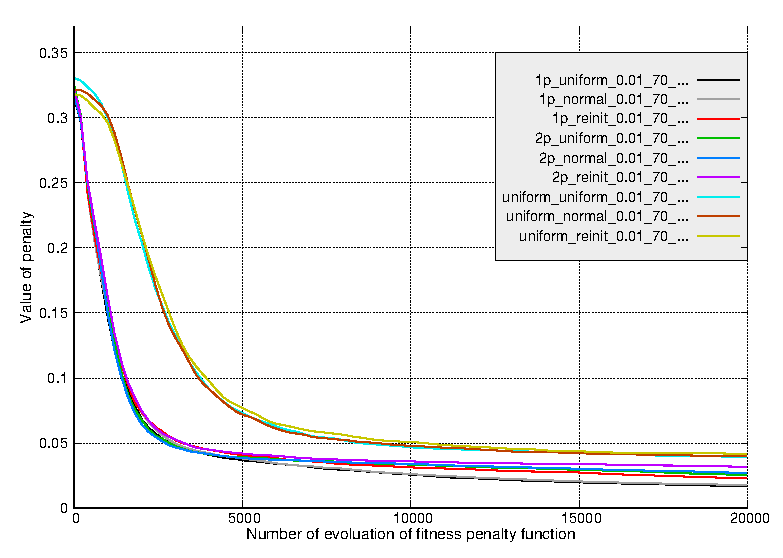
\includegraphics[width=5.0in]{operators_comparison}
    \caption{Comparison of crossover operators types with mutation operator types}
    \label{operatorcomparison}
\end{figure}

\begin{figure}
    \centering
    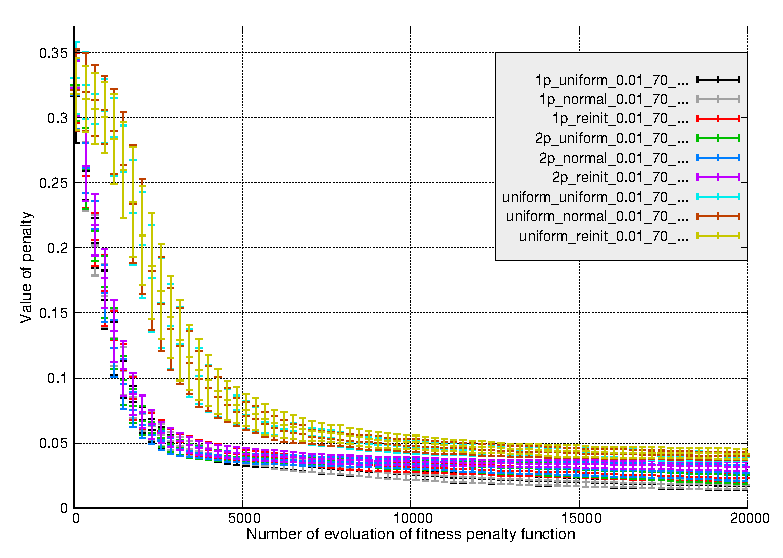
\includegraphics[width=5.0in]{operators_comparison_err}
    \caption{Comparison of crossover operators types with mutation operator types, standard deviation.}
    \label{operatorcomparisonerr}
\end{figure}

\begin{figure}
    \centering
    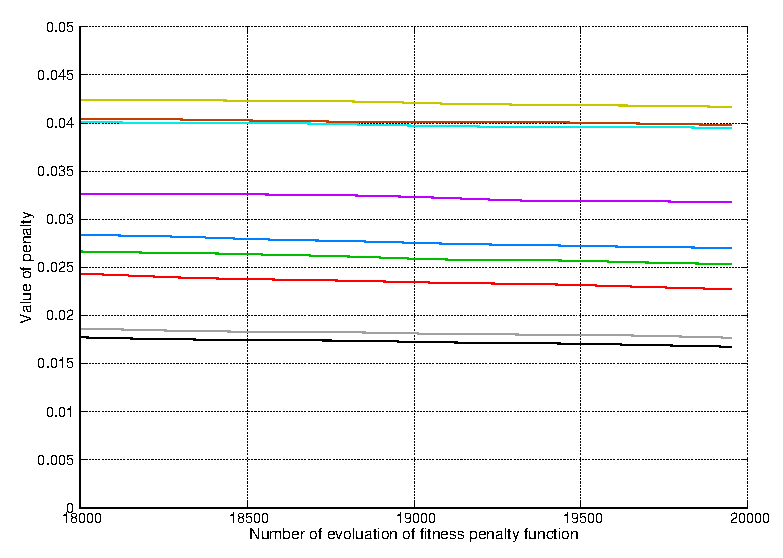
\includegraphics[width=5.0in]{operators_comparison_zoom}
    \caption{Comparison of crossover operators types with mutation operator types, zoomed to the end interval of graph.}
    \label{operatorcomparisonzoom}
\end{figure}

The next pair of parameters are mutation probability and population size. This pair is much more complicated because now there are no discrete values for parameters and one needs to find optimal value for continuous space. In frame of current study the search of optimal solution will be quite primitive and more complitated methods are remained for further researches. The search strategy will be done in following manner. For each parameter of pair some discrete values are chosen. For each value among chosen discrete parameters computations are performed. From obtained data fitting function is founded and all other comparison of parameters made based on fitted function.

Just for visual comparison, Figure \ref{mppscomparison001}, Figure \ref{mppscomparison01}, Figure \ref{mppscomparison08} show dependency of mutation probability on population size. Figure \ref{mppscomparison001} shows fixed mutation probability equal to 0.01 and different population size, Figure \ref{mppscomparison01} - mutation probability 0.1, Figure \ref{mppscomparison08} - mutation probability 0.8. It is presented only little part of studied data, just for visualization of dependency.

\begin{figure}
    \centering
    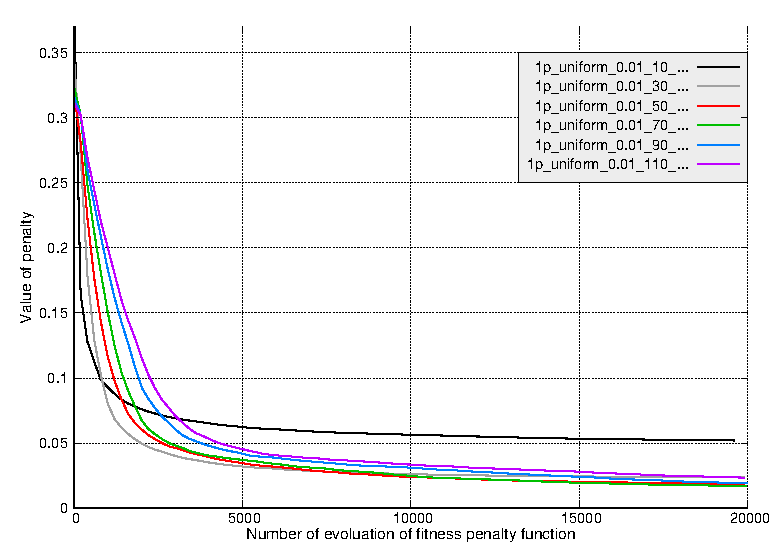
\includegraphics[width=5.0in]{mppscomparison001}
    \caption{Comparison of fixed mutation probability 0.01 and different population size}
    \label{mppscomparison001}
\end{figure}

\begin{figure}
    \centering
    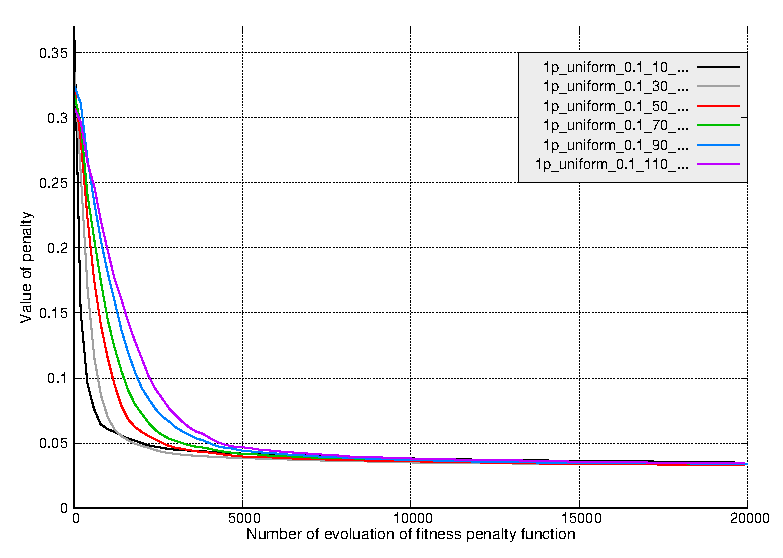
\includegraphics[width=5.0in]{mppscomparison01}
    \caption{Comparison of fixed mutation probability 0.1 and different population size}
    \label{mppscomparison01}
\end{figure}

\begin{figure}
    \centering
    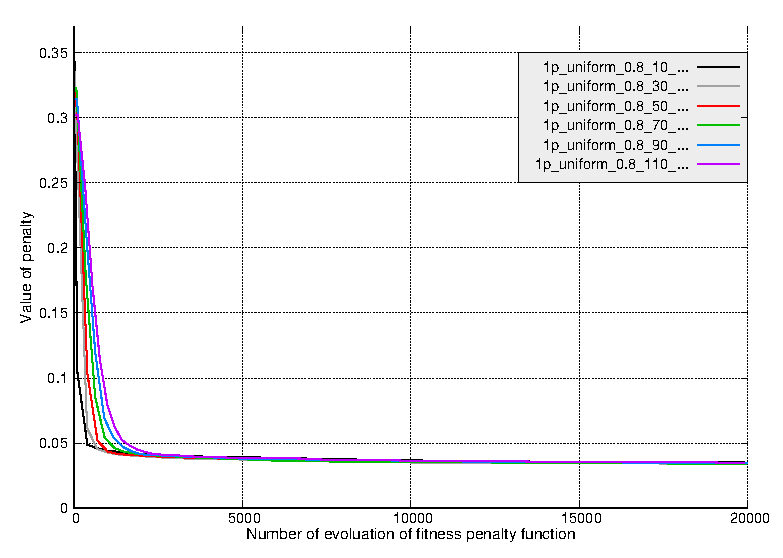
\includegraphics[width=5.0in]{mppscomparison08}
    \caption{Comparison of fixed mutation probability 0.8 and different population size}
    \label{mppscomparison08}
\end{figure}

For quantative comparison GA with different values of mutation probabilty and population size, and finding of optimal combintation it is needed to fit data to some function. After series of experiments it was decided to divide data to 2 parts and fit these 2 parts with different functions. First part is in iterval [0, 3500] and the second part from 3500 till the end of data. For the first interval the fitting function is: 

\begin{equation} \label{sig1}
sig_1(x) = \frac{a}{b+x^d}+c
\end{equation}
\bigbreak

And for the second interval is:

\begin{equation} \label{sig2}
sig_2(x) = \frac{a}{b+x}+c
\end{equation}
\bigbreak

So, the task is to find a, b, c, d parameters for the above functions. The results after fitting  can be found in the appendix and there are  presented just the best result. Before analysis of the result it is needed to understand how one can compare different obtained functions and say that one is better then another for the current task. The best solution is to invent a measure for functions. The idea was accepted: first interval shows how fast is convergence of configuration and the second interval shows whether configuration converges. For measuring speed of convergence the average velocity on interval was considered:

\begin{equation} \label{mes1}
mes_1(sig_1(x)) = \frac{sig_1(x_{start}) - sig_1({x_{end}})}{3500}
\end{equation}
\bigbreak
 
where $x_{start}$ is first point of interval $x_{end}$ is end point of interval, 3500 was chosen because it is length of the interval.

And for the second interval just parameter c was condered as a measure because it is limit point for Formula \ref{sig2} when $x \rightarrow \infty$:

\begin{equation} \label{mes2}
mes_2(sig_2(x)) = \lim_{x\to\infty} sig_2(x) = \lim_{x\to\infty}  \frac{a}{b+x}+c = c
\end{equation}
\bigbreak

The surface showing dependency of first measure on mutation probability and population size is shown on Figure \ref{speedsurface} and dependency of GA limit value on the same parameters is shown on Figure \ref{limitsurface}

\begin{figure}
    \centering
    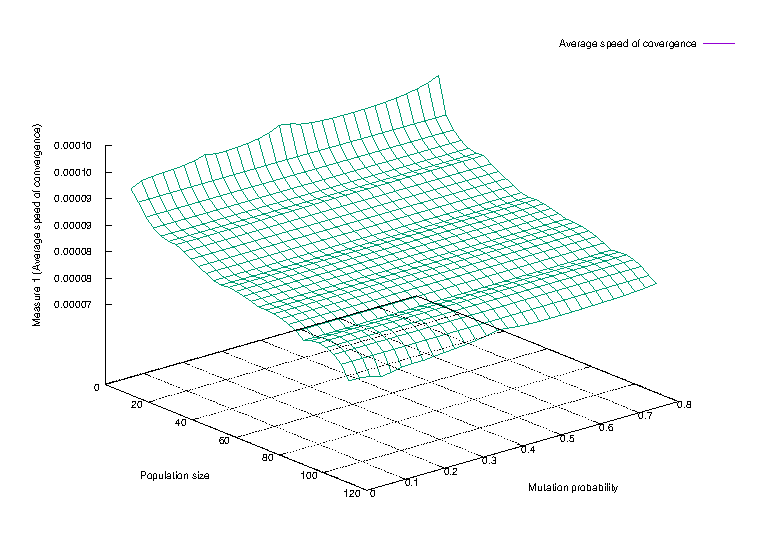
\includegraphics[width=5.0in]{speed_surface}
    \caption{Average evolution rate dependency on mutation probability and population size}
    \label{speedsurface}
\end{figure}

\begin{figure}
    \centering
    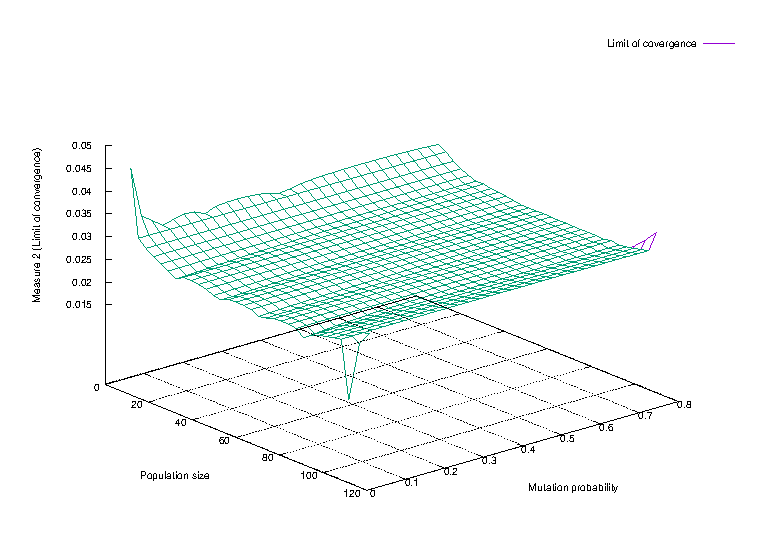
\includegraphics[width=5.0in]{limit_surface}
    \caption{Limit of convergence dependency on mutation probability and population size}
    \label{limitsurface}
\end{figure}

As one can see, evolution rate is higher on small populations. And limit is lower (better convergence) on big populations. The best result according to the first measure showed configuration with mutation probability - 0.8 and population size - 10. It means that with such a configuration GA converges faster, at least in the very beginning of algorithm run. But for the best convergence value the best configuration is mutation probability - 0.01 and population size - 90, i.e. the configuration has lower limit. Such different behavior in different configuration prompted to extend method used in one of mentioned papers \ref{
shen15} and use it for the current task.

The idea of thresholds was a decision for the problem how to combine results for different configurations. The meaning of the approach is to change mutation probablity and population size when algorithm reach number of runs equal to threshold. This idea can be extended to many numbers of thresholds but in this work it was limited by only two thresholds.

First step of optimization of thresholds was done by changing the first threshold and second thresholds but keeping difference between them the same and equal to 100 runs. The result is shown on Figure \ref{threshold1comparison}. As one can notice while first threshold is equal to 200 the GA has best result in penalty. Notice, labels again shortened. But now they are shortened from both sides start and end. The third shown parameter in the labels is first threshold while fourth - second threshold.

\begin{figure}
    \centering
    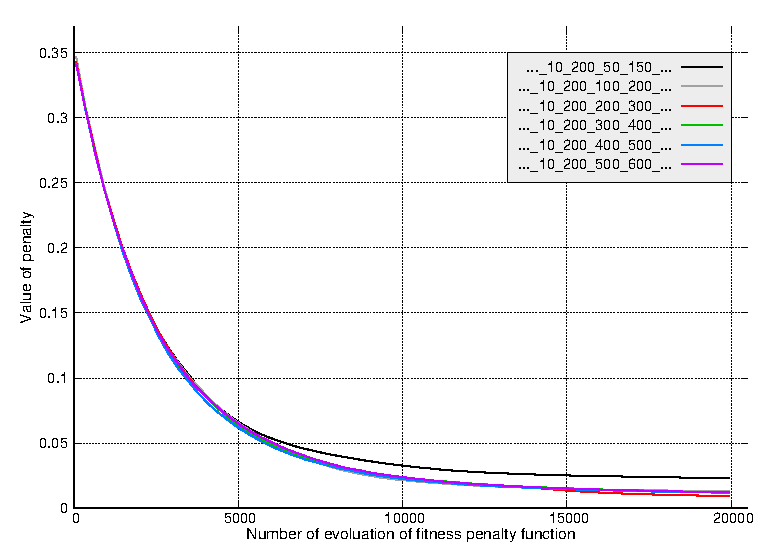
\includegraphics[width=5.0in]{threshold1_comparison}
    \caption{Comparison of different values of first threshold while second threshold is fixed}
    \label{threshold1comparison}
\end{figure}

Second step of optimization of thresholds was done by fixing first threshold equal to 200 (see previous result) and changing difference between thresholds. The result is shown on Figure \ref{threshold2comparison}. As one can notice, the results are very similar to each other, but in this work threshold equal to 500 was chosen.

\begin{figure}
    \centering
    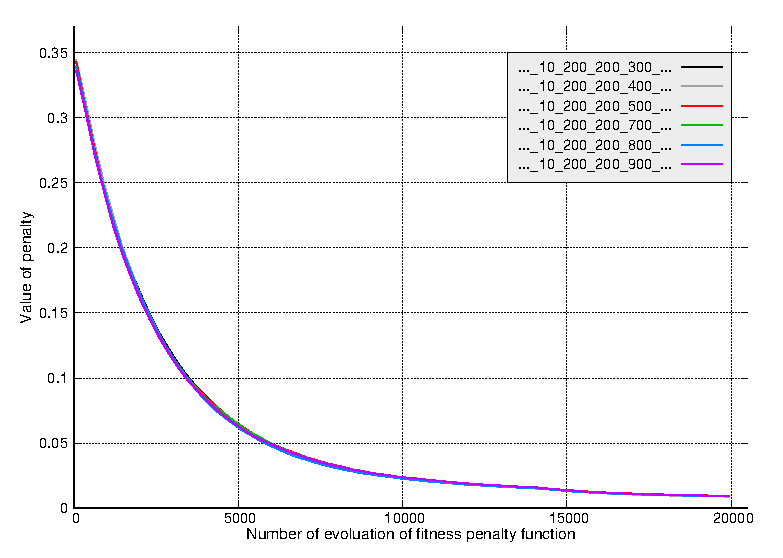
\includegraphics[width=5.0in]{threshold2_comparison}
    \caption{Comparison of different values of second threshold while first threshold is fixed and equal to 200}
    \label{threshold2comparison}
\end{figure}

Of course these threshold parameters could be optimized more seriously but it goes away from the current work. The rest parameters remained as it was declared previously for default values.

After having the optimal configuration, 1000 of session on such configuration were run in order to obtain the best fitted Voronoi structure and statistics for the configuration. The result of fitting is presented on Figure \iffalse \ref{lastconvergence} \fi  for convergence and on Figure \iffalse \ref{lastresult} \fi for comparison size distribution before GA application and after. During run, penalty reduced 1000 times compared to the initial distribution.
On Figure \iffalse \ref{lastconvergence} \fi 3 lines are presented: the best individual's penalty, the worst individual's penalty and the average penalty for the number of evaluating of penalty function.


\subsection{Building the Voronoi tessellation fitting the given grain orientation distribution}

Firsty, it is needed to understand why grain orientation distribution is so important. Different orientation of neighboring grains leads to the grain boundary appearing. Boundary, in its turn, is very important because:

- Grain boundary vary significantly in their characteristics compared to bulk material (mobility, energy, chemistry)

- Many properties of material depend on the nature of grain boundaries (electrical resistance, strain-stress properties, chemical properties etc)

- Material can have good or bad mechanical, corrosion properties depending on the type of grain boundaries
  
One of the popular method to represent the grain distribution is to calculate distribution of misorientation angles between neighboring grains. Given two orientations (grains, crystals), the misorientation is the transformation required to transform tensor quantities (vectors, stress, strain) from one set of crystal axes to the other set. For cubic lattice (in current study comparison will be for experimental data for FCC materials) there are 24 variants of rotation (transformation) that can transform one grain to another. But for misorientation distribution we need only lowest angle of misorientation. To calculate misorientation one need to know Euler angles of neighboring grains. For each grain with Euler angles [$\phi_1, \Phi, \phi_2$] it is needed to calculate orientation matrix:

\begin{equation} \label{orientmatrix}
g = \begin{bmatrix}
    c\phi_1c\phi_2 - s\phi_1s\phi_2c\Phi & s\phi_1c\phi_2 - c\phi_1s\phi_2c\Phi & s\phi_2c\Phi \\
    -c\phi_1s\phi_2 - s\phi_1c\phi_2c\Phi & -s\phi_1s\phi_2 - c\phi_1c\phi_2c\Phi & c\phi_2s\Phi \\
    s\phi_1s\Phi & -c\phi_2s\Phi & c\Phi
\end{bmatrix}
\end{equation}
\bigbreak

where c is cos, s is sin.

The misorientation matrix is then:

\begin{equation} \label{mismatrix}
\Delta g_{1,2} = g_1A_{rot_i}g^{-1}_2
\end{equation}
\bigbreak

where $g_1$ is orientation matrix for the first grain, $g_2$ is orientation matrix for the second grain and $g^{-1}_2$ is invert matrix for $g_2$, $A_{rot_i}$ is i-th rotation matrix (there are 24 of them, see appendix).

And from misorientation matrix it is possible to calculate misorientation angle:

\begin{equation} \label{misangle}
cos\Theta = (trace(\Delta g_{1,2}) - 1)/2
\end{equation}
\bigbreak

From 24 matrices one obtain 24 angles, but only smallest is valid for distribution.

There are many different misorientation angle distributions. The shape of distributions for different type of lattice can be found in Hans Grimmer's paper \cite{hans79}. But currently in the work just cubic lattice is beeing considered. This is why Mackenzie distribution \cite{mack58} is taken as a primary distribution for this study. It does not mean that only this distribution is possible to reach in frame of current work. The framework is able to fit any user defined distribution. But Mackenzie distribution is taken as a reference for initial research. 

Default random grain orientation distribution is described by Mackenzie distribution. This is why when one generate grain orientation randomly and even pseudo-randomly one obtain distribution very close the Mackenzie distribution. In order to check if implemented algorith works with any kind of initial grain orientation distributions, the initial orientations selection algorithm was changed. Initial orientation selection is based on generating Euler angles within [0\degree, 9\degree] interval. This algorithm generates \textit{\textbf{texture}} in simulated structure. The \textit{\textbf{texture}} for polycrytalline is orientation distribution with some prefered direction.

As one can understand, for fitness penalty calculation in this algorithm Mackenzie function was used. But what about other key elements of GA for orientation distribution? 

Individual for this implementation is Voronoi structure obtained in previous grain size algorithm with some specified orientation of lattice, i.e. 3 Euler angles. To create first population some specified number of individuals with random Euler angles is generated.

Crossover operator works here similarly to previos implementation in grain size algorithm, but instead of interchanging seeds, operator interchanges Euler angles between two individuals. Exchange is made by simple interchange of angels of two corresponding individuals' seeds. Because seeds in all individuals are the same and fixed, the exchange algorithm is pretty simple interchanging angles between seeds positioned on the same coordinates.

Mutation operator works here by just simple slight changing of angles. Because in this study for now only cubic lattice is considered, one can limit all angles by 90 degree. It is possible due to cubic symmetry in the lattice. Thank to this property it is possible to determine fixed shifting parameter for mutation operator. Here it is k*90/100 degree, where k is coefficient defined as parameter in order to be able to control amplitude of shifting and find some optimal value.

All the rest elements of GA here are implemented absolutely similarly to GA for grain size. The set of parameters is the same and therefore it needs 



[ToDo] describe elements for GA of orientation

[ToDo] show comparison of different pairs and configs

[ToDo] show result for best configuration


\section{Filling tessellation with particles (atoms)}

After getting correct container for polycrystalline and getting orientations of grains (in Euler angles) one can fill the container by atoms. Atoms should follow specified lattice, and lattice has to be defined by base atoms. In general, any of possible lattices can be defined in code, but in this work only cubic structures are considered.

The process of lattice generation is pretty simple. The grain's seed point is considered as a starting point for lattice generation. Atoms located in oX, oY, oZ directions with lattice constant periodicity starting from this point. The distance between starting point and last atoms in each directions is of diameter of the grain. After generating none-rotated lattice it is needed to rotate it according to the Euler angles obtained in previous step. It is done straightforward according to the defenition of Euler angles. 

After rotation one needs to remove excess atoms that stay outside of the grain volume. This procedure is done in this way: for all planes of grain coefficients of the plane's equation are calculated ($Ax + By + Cz = D$), then for the seed point with coordinates $(x_1, y_1, z_1)$ signs for each plane of grain are calculated ($Ax_1 + By_1 + Cz_1 - D$), and the process repeated for all atoms of generated lattice. When even one sign differs from the sign of the seed then this atom lie outside of grain volume and need to be deleted.

It is important to notice that if the generated lattice will be moved in any axis by distance equal to lattice constant then we obtain absolutelly similar position of atoms (inside of grain because of periodicity of lattice) but we still get different position of atoms if we shift lattice by distance less then lattice constant. This feature will be used during first step of relaxation and this possible shifting is called \textit{\textbf{shifting vector}} in current study. So, finally for each grain one got 9 parameters: 3 coordinates of seed, 3 coordinates of shifting vector, 3 Euler angles. The result population of grains with atoms one can see on Figure \ref{cubefilled}

\begin{figure}
    \centering
    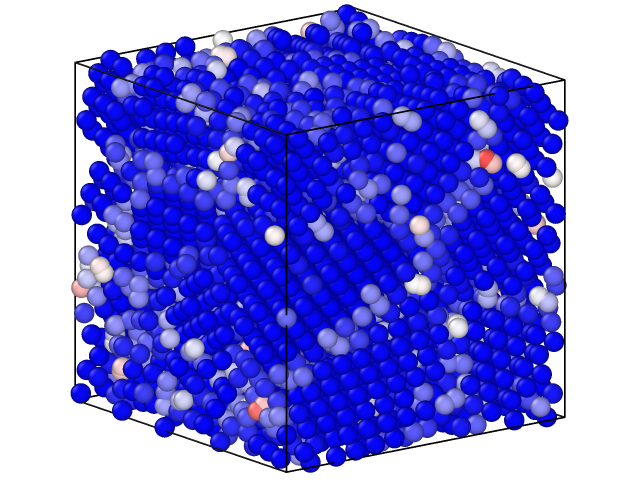
\includegraphics[width=5.0in]{cube_filled}
    \caption{Voronoi tessallation with filled grains}
    \label{cubefilled}
\end{figure}

\section{Relaxation of atomic structure}

As well known, the nature acts in such a way that any body tends to energy minimization in order to exist. Therefore in order to obtain realistic structure one needs to minimize energy of the system. In case of current work it is needed to find such positions of atoms which provide minimum potential energy of whole atoms set.

The process of energy minimization is called relaxation of the system. In current work relaxation is made in two steps. First step involved genetic algorithm for grain atoms shifting and second one is about removing high tension atoms. By saying high tension one means atoms which bring positive or not enough negative value of potential energy to the system.

In this work Embeded Atom Method (EAM) is used for system energy calculation (see Appendix Figure \ref{eamappendix}. For the test purpose aluminum is taken as a reference element for properties checking. 

All energy calculations are done by using LAMMPS software build as a static library for linux system.

\subsection{Relaxation by grain atoms shifting}

As was mentioned, this is the first step of relaxation process. This approach is possible because of not ideal positioning of generated atoms for each grain. One can find that by shifting all atoms of grain one can increase or decrease energy of the system. This happens because shifting leads to increasing distances between atoms on some boundaries and decreasing distances on another boundaries. The aim of relaxation is to find optimal shifting for all grains. For this purpose genetic algorithm again in use. In this work "shifting relaxation" phrase is used to point this kind of relaxation.

Genetic algorithm for atoms shifting is based on the same principles as was discussed above for grain size and grain orientation. The same process of finding optimal configuration is done for this algorithm. 

[ToDo] show results for optimal configuration finding for the shifting

\subsection{Relaxation by removing excess atoms}

Despite shifting relaxation some atoms have very high potential energy (on the boundary), sometime even positive value. This leads to unreasonable values of total energy of the system. Sometimes structure even could not exist in nature with such high values of energy and therefore one needs to remove such atoms if there are no another methods to relax the system.

In order to understand what atoms are excess and needed to be removed one have to introduce some criteria or measure that will show how "bad" or "good" is atom. In this work the simple criteria of potential energy of the atom is used. Partucularly, one can define some threshold for energy and remove all atoms exceeding this value of energy. The logically simplest threshold value is 0. If atom exceeds this energy (i.e. has positive energy contribution) then atom can be removed. The example result for such threshold is presented on Figures \ref{cubefilled} and \ref{cubefilled}.

The process of excess atom removing is iterative. After removing of candidate atom total energy recalculation is needed. Because dependency of total energy is not linear in EAM it is difficult to predict how atom removal will affect to total energy of the system. If after atom removal total energy decreases this system alteration is accepted and next atom can be considered. Note, that after each atom removal it is needed to recalculate energies for all atoms and start "bad" atoms search from scratch, because it is hard to predict how removal will change energy of all atoms. The process continues until having all atoms with energy less or equal to the threshold value.


[ToDo] show graphs for energy dumping for different thresholds

\subsection{Relaxation by molecular static minimization}

The next two steps of relaxation is out of the current program module and done just to complete the relaxation process. In reality researcher has to do this by himself in LAMMPS software or any another program suitable for molecular statics and molecular dynamics.

The first step is searching of optimized size of simulation volume and position of atoms. For this purpose "minimize" LAMMPS command is used. The process done in loop in order to get deep optimal result. In each iteration firstly, relaxation of the simulation box performed, then only relaxation of particles' coordinates is done. Atfer several iteration one obtains staticaly relaxed structure.

\subsection{Relaxation by molecular dynamics}

The last step in relaxation process is molecular dynamics simulation. This step is done with the same LAMMPS software. 

\section{Conclusion}

During this work the main aim of the study was done - the tool for realistic polycrystalline structure generation was created. This tool has its own pros and cons. No one can guarantee that such a structure will fit any polycrystalline structures in nature. Especially if one talks about sameness of grains. Voronoi tesselation cannot generate non-convex structures and is not allowing to have non-linear boundaries. But nonetheless, this method can help to simulate many of natural structures with precision enough for many properties. It is also needed some extra manupulation with multi-type atom structure. One need to be carefull about neutral charge of the system. Nevertheless, this tool provides very flexible and powerfull mechanism for obtaining close to experimental data polycrystalline structure. One needs just define grain size, grain orientation distributions, lattice constant, lattice base, prefered simulation box and just run the program. As a result one will get ready to use structure in LAMMPS output format.

Next step in this study might be universalization of algorithm in order to allow it to simulate more broad structures. Add pre-refinement such as Laguere-Voronoi tessellation which will allow to get structure very close to the given distribution in the very beginning of algorithm and will reduce total calculation time. There are few others approaches that will help with orientation distribution pre-refinement and with atom filling algorithms. They can help in further studies based on current tool.

Make it more userfriendly. This tool should have console version like regular scientific application and allow users to interact with program via some commands. This is one of the directions of tool impovement.

Add more detailed documentation and integrate different input and output formats. For now user has to define distibution functions in code and compile it in order to get some usable binary to generate necessary structure. It would be much more convenient to define functions as an input for console parameters or even to locate some file with functions where program can read data and operate with it during structure generation. The same situation with output of results. Currently, only LAMMPS trajectory file is supported as output format. But it is needed to broaden available output formats.

Among possible program extension genetic algorithm parameters manual control possibility might be considered. User has to have potential to control all about genetic algorithm in order to find parameters more suitable for user's case.

\section{Acknowlegments}

Financial support of the MathMods Erasmus Mundus program and especially prof. Bruno Rubino is gratefully acknowledged. Prof. Szymon Winczewski is aknowledged for his professional and careful supervision of this master thesis. M.Sc.Eng. Kamil Rybacki is aknowledged for his support in many issues during implementation of the software for the current research. Dr. eng. Karol Frydrych is acknowledged for suggestion how to calculate misorienation angle. Dr. Anton Pshenichnikov is aknowledged for suggestion about relaxation of the structure. Special acknowlegments for Gdansk University of Technology for providing access to the supercomputer.

\goodbreak
\section{Appendix}

[ToDo] show results of fitting data of params to the function

[ToDo] show genotype to phenotype encoding

[ToDo] give link to the repo

\begin{figure}
    \centering
    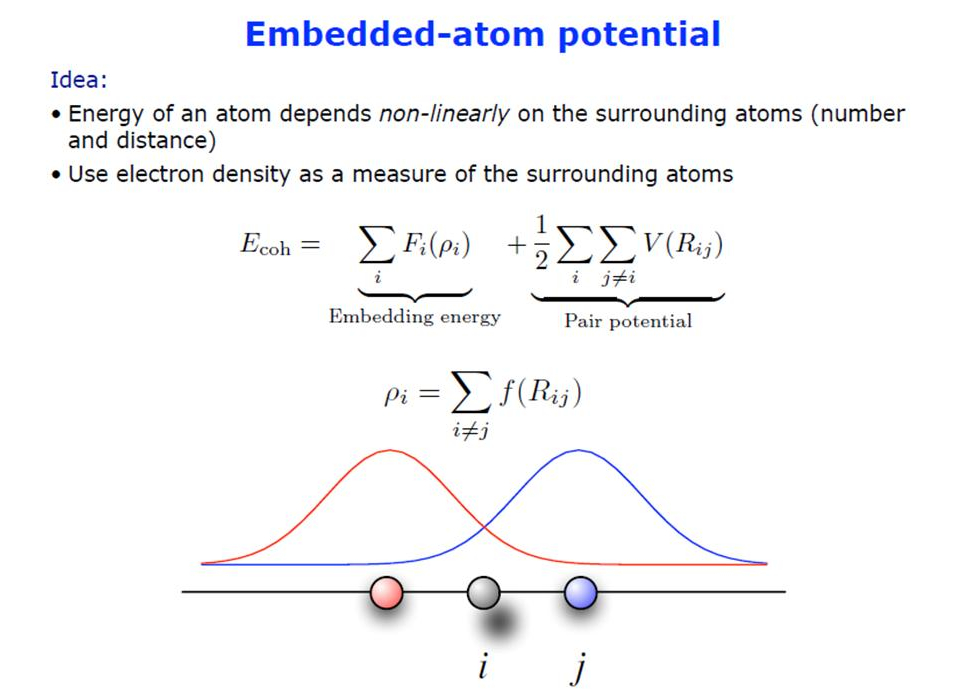
\includegraphics[width=5.0in]{EAM_appendix}
    \caption{Main idea of Embeded Atom Model potential}
    \label{eamappendix}
\end{figure}

\begin{figure}
    \centering
    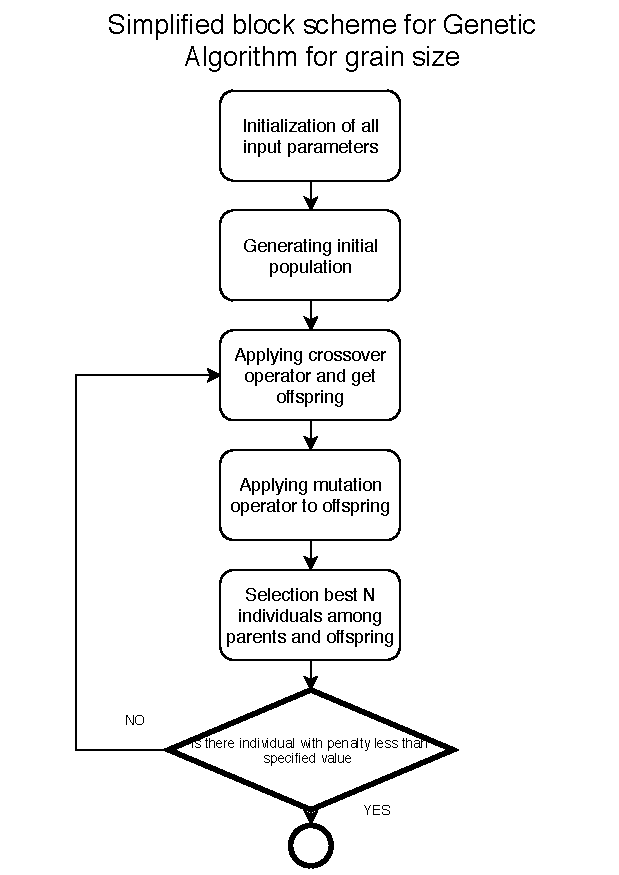
\includegraphics[width=5.0in]{grain_size_blockscheme}
    \caption{Grain size block scheme. Also valid for any genetic algorithm used in this work.}
    \label{grainsizeblock}
\end{figure}

\begin{figure}
    \centering
    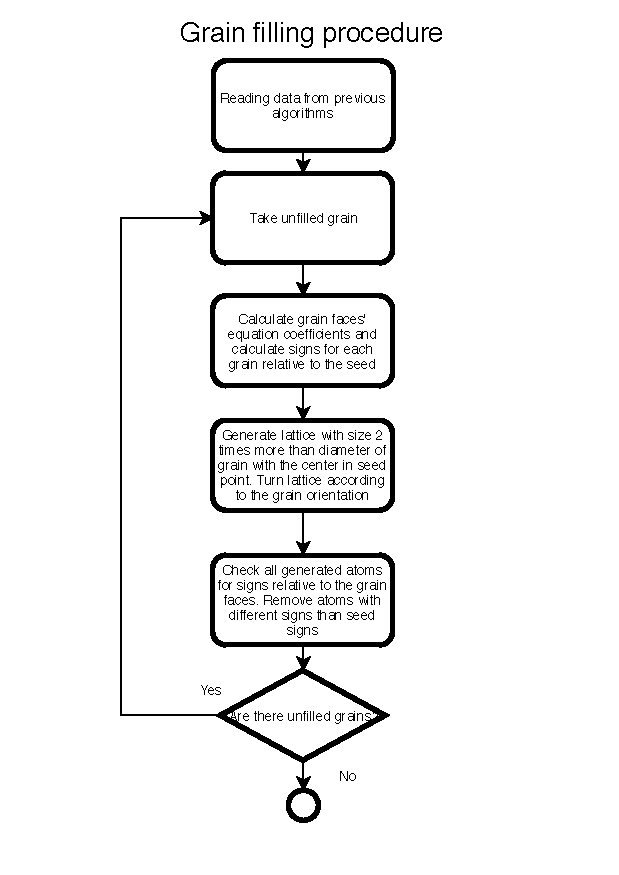
\includegraphics[width=5.0in]{GrainFillingScheme}
    \caption{Grain filling procedure's block scheme}
    \label{grainfillingblock}
\end{figure}

\begin{figure}
    \centering
    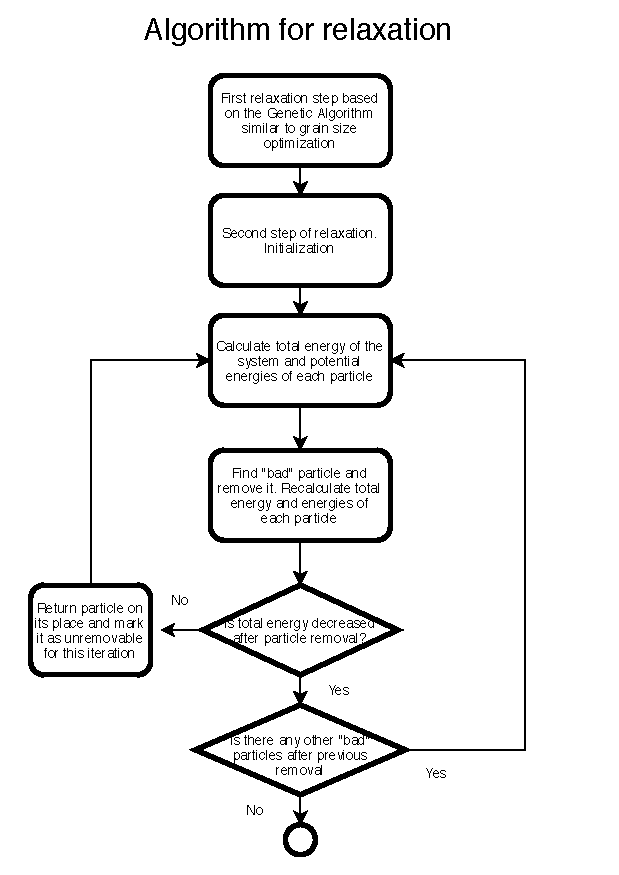
\includegraphics[width=5.0in]{RelaxationCommonBlockScheme}
    \caption{Relaxation algorithm block scheme}
    \label{relaxation block}
\end{figure}



\begin{thebibliography}{9}

\bibitem{john99}
  Johnson C. E. J.
  \textit{Tritium behavior in lithium ceramics}
  Nucl. Mater
  1999

\bibitem{pardo11}
  Pardo, Lorena, Ricote, Jesús (Eds.)
  \textit{Multifunctional Polycrystalline Ferroelectric Materials}
  Springer
  2011

\bibitem{schrop98}
  Schropp, Ruud E. I. Zeman, Miro
  \textit{Amorphous and microcrystalline silicon solar cells : modeling, materials, and device technology}
  Boston (Mass.) : Kluwer academic
  1998.

\bibitem{harb85}
   Harbeke, G. (Ed.)
  \textit{Polycrystalline Semiconductors}
  Springer-Verlag Berlin Heidelberg
  1985

\bibitem{plimp95}
   S. Plimpton 
  \textit{Fast Parallel Algorithms for Short-Range Molecular Dynamics}
  J Comp Phys, 117, 1-19
  1995

\bibitem{plimp00}
   S. Plimpton 
  \textit{LAMMPS WWW Site}
  http://lammps.sandia.gov

\bibitem{shen15}
  Shen, Y. et al. 
  \textit{Constructing three-dimensional (3D) nanocrystalline models of Li4SiO4 for numerical modeling and simulation.}
  Sci. Rep. 5, 10698; doi: 10.1038/srep10698 
  2015

\bibitem{terada10}
  D Terada et al.
  \textit{Effect of grain size distribution on mechanical properties of ultrafine grained Al severely deformed by ARB process and subsequently annealed}
  2010 J. Phys.: Conf. Ser. 240 012111


\bibitem{suzudo02}
  Suzudo T.  Kaburaki H. 
  \textit{An evolutional approach to the numerical construction of polycrystalline structures using the Voronoi tessellation}
  Phys. Lett. A 373, 4484–4488 (2009).

\bibitem{wang96}
  Wang J. et al. 
  \textit{Computer simulation of the structure and thermo-elastic properties of a model nanocrystalline material}
  Philos. Mag. A. 73, 517–555 
  1996

\bibitem{rinaldi08}
  Antonio Rinaldi, Dusan Krajcinovic, Pedro Peralta, Ying-Cheng Lai
  \textit{Lattice models of polycrystalline microstructures: A quantitative approach}
  Mechanics of Materials 40 (2008) 17–36

\bibitem{hans79}
  Hans Grimmer
  \textit{The distribution of disorientation angles if all relative orientations of neighbouring grains are equally probable}
  Scripta Metallurgica
Volume 13, Issue 2, February 1979, Pages 161-164

\bibitem{mack58}
  Mackenzie, J.K.
  \textit{Second Paper on the Statistics Associated with the Random Disorientation of Cubes}
  Biometrika 45,229.
 (1958)

\bibitem{kotak12}
  Jani Kotakoski and Jannik C. Meyer
  \textit{Mechanical properties of polycrystalline graphene based on a realistic atomistic model}
  Phys. Rev. B 85, 195447 – 24 May 2012

\bibitem{guo13}
  Guo-Jie J. Gao  Yun-Jiang Wang Shigenobu Ogata
  \textit{Studying the elastic properties of nanocrystalline copper using a model of randomly packed uniform grains}
 Computational Materials Science
Volume 79, November 2013, Pages 56-62

\bibitem{prak16}
  A.Prakash M.Hummel S.Schmauder E.Bitzeka
  \textit{Nanosculpt: A methodology for generating complex realistic configurations for atomistic simulations}
 MethodsX
Volume 3, 2016, Pages 219-230

\bibitem{juli03}
  Ju Li
  \textit{AtomEye: an efficient atomistic configuration viewer}
 Modelling Simul. Mater. Sci. Eng. 11 (2003) 173–177

\bibitem{hirel15}
  Pierre Hirel
  \textit{Atomsk: A tool for manipulating and converting atomic data files}
 Computer Physics Communications
Volume 197, December 2015, Pages 212-219

\bibitem{falco15}
  SimoneFalco JiaweiJian Francesco De Cola Nik Petrinic
  \textit{Generation of 3D polycrystalline microstructures with a conditioned Laguerre-Voronoi tessellation technique}
 Computational Materials Science
Volume 136, August 2017, Pages 20-28


\bibitem{wear86}
  Weaire D. et al. 
  \textit{On the distribution of cell areas in a Voronoi network}
  Philos. Mag. B 53, 101–105 
  1986

\bibitem{fan04}
  Fan Z. G. et al. 
  \textit{Simulation of polycrystalline structure with Voronoi diagram in Laguerre geometry    based on random closed packing of spheres} 
  Comput. Mater. Sci. 29, 301–308 
  2004

\bibitem{okabe00}
Okabe A. et al. 
\textit{Spatial Tessellations-Concepts and Applications of Voronoi Diagrams}
Wiley, New York, 
2000

\bibitem{sivan98}
  S. N. Sivanandam , S. N. Deepa
  \textit{Introduction to Genetic Algorithms},
  Springer Publishing Company, Incorporated
  2007

\bibitem{melan98}
  Melanie Mitchell
  \textit{An Introduction to Genetic Algorithms}
  MIT Press, Cambridge, MA
 1998

\bibitem{gold06}
  David E. Goldberg
  \textit{Genetic Algorithms}
  Pearson Education, 2006

\bibitem{suwas14}
  S. Suwas and R. K. Ray
  \textit{Crystallographic Texture of Materials}
  Springer-Verlag London 
  2014

\bibitem{liu14}
  Xuan Liu, Andrew P. Warren,
  \textit{Comparison of crystal orientation mapping-based and image-based measurement of grain size and grain size distribution in a thin aluminum film}
  Acta Materialia 79, 138–145
  2014

\end{thebibliography}


\end{document}
